% =====================================================================
%  Observatorio MinCiencias — Informe consolidado
%  Universidad Santo Tomás · Ustadistica · 2026-I
%
%  Compilación recomendada (UTF-8):
%      pdflatex informe_final.tex
%      pdflatex informe_final.tex     % segunda pasada para referencias
%
%  Alternativas:
%      xelatex informe_final.tex
%      tectonic informe_final.tex
%
%  Las figuras se cargan desde ../../artifacts/sprint*/  (paths relativos)
% =====================================================================

\documentclass[11pt,a4paper,oneside]{article}

% ---- Codificación e idioma -----------------------------------------
\usepackage[utf8]{inputenc}
\usepackage[T1]{fontenc}
\usepackage[spanish,es-tabla,es-lcroman]{babel}
\usepackage{lmodern}
\usepackage{microtype}

% ---- Geometría y tipografía ----------------------------------------
\usepackage[a4paper,top=2.6cm,bottom=2.6cm,left=2.7cm,right=2.7cm]{geometry}
\usepackage{setspace}
\setstretch{1.18}
\usepackage{parskip}

% ---- Colores y enlaces ---------------------------------------------
\usepackage{xcolor}
\definecolor{usta}{RGB}{30,55,128}
\definecolor{accent}{RGB}{183,135,30}
\definecolor{rule}{RGB}{170,170,170}
\definecolor{soft}{RGB}{245,245,247}
\usepackage[colorlinks=true,linkcolor=usta,citecolor=usta,urlcolor=usta]{hyperref}

% ---- Figuras y tablas ----------------------------------------------
\usepackage{graphicx}
\usepackage{caption}
\captionsetup{font=small,labelfont=bf,labelsep=period,justification=raggedright,singlelinecheck=false}
\usepackage{booktabs}
\usepackage{siunitx}
\sisetup{output-decimal-marker={,},group-separator={.},group-minimum-digits=4}
\usepackage{array}
\usepackage{tabularx}
\usepackage{multirow}

% ---- Listas --------------------------------------------------------
\usepackage{enumitem}
\setlist{itemsep=2pt,topsep=4pt,parsep=0pt}
\usepackage{epigraph}
\setlength{\epigraphwidth}{0.65\textwidth}

% ---- Encabezados de sección ---------------------------------------
\usepackage{titlesec}
\titleformat{\section}
  {\Large\bfseries\color{usta}}{\thesection}{0.7em}{}[\vspace{-0.2em}\color{rule}\hrule]
\titleformat{\subsection}
  {\large\bfseries}{\thesubsection}{0.6em}{}
\titleformat{\subsubsection}
  {\normalsize\bfseries\color{usta!85}}{\thesubsubsection}{0.5em}{}
\titlespacing*{\section}{0pt}{1.6em}{0.6em}
\titlespacing*{\subsection}{0pt}{1.0em}{0.4em}

% ---- Encabezado y pie ----------------------------------------------
\usepackage{fancyhdr}
\pagestyle{fancy}
\fancyhf{}
\renewcommand{\headrulewidth}{0pt}
\fancyfoot[L]{\footnotesize\color{rule} Observatorio MinCiencias \,$\cdot$\, USTA \,$\cdot$\, 2026-I}
\fancyfoot[R]{\footnotesize\color{rule}\thepage}

% ---- Recuadros -----------------------------------------------------
\usepackage[most]{tcolorbox}
\tcbset{
  hallazgo/.style={
    enhanced, colback=soft, colframe=accent, boxrule=0.6pt, arc=2pt,
    left=10pt, right=10pt, top=8pt, bottom=8pt, fontupper=\small,
  },
  caveat/.style={
    enhanced, colback=white, colframe=usta!50, boxrule=0.4pt, arc=2pt,
    left=10pt, right=10pt, top=6pt, bottom=6pt, fontupper=\footnotesize,
  }
}
\newtcolorbox{hallazgo}{hallazgo}
\newtcolorbox{caveat}{caveat}

% ---- Código --------------------------------------------------------
\usepackage{listings}
\lstset{
  basicstyle=\ttfamily\footnotesize,
  backgroundcolor=\color{soft},
  frame=single, framerule=0pt, rulecolor=\color{rule},
  breaklines=true, showstringspaces=false,
  keywordstyle=\color{usta}\bfseries,
  commentstyle=\color{rule}\itshape,
  stringstyle=\color{accent},
  numbers=none, language=Python,
  xleftmargin=8pt, xrightmargin=8pt,
}

% ---- Metadatos editables -------------------------------------------
\newcommand{\autorInforme}{Víctor Díaz Bautista}
\newcommand{\directorInforme}{Iván Zainea}
\newcommand{\universidad}{Universidad Santo Tomás}
\newcommand{\unidad}{Ustadistica \,$\cdot$\, Consultoría e Investigación}
\newcommand{\periodo}{2026-I}
\newcommand{\repoUrl}{https://github.com/Victor-Diaz-Usta/Min\_ciencias}

\title{}
\author{}
\date{}

% =====================================================================
\begin{document}
% =====================================================================

% ---- PORTADA -------------------------------------------------------
\begin{titlepage}
\thispagestyle{empty}
\centering
\vspace*{1.4cm}
{\footnotesize\sffamily\color{rule}\universidad\\\unidad\\\periodo}\par
\vspace{2.2cm}
{\Huge\bfseries\color{usta} El sistema de reconocimiento\\[2pt] de investigadores en Colombia}\par
\vspace{0.8cm}
{\Large\itshape Auditoría sobre seis convocatorias de MinCiencias\\(2013--2021)}\par
\vspace{2.4cm}

{\color{accent}\rule{0.4\linewidth}{0.6pt}}

\vspace{0.8cm}
\begin{tabularx}{0.7\linewidth}{>{\raggedright\arraybackslash}X >{\raggedleft\arraybackslash}X}
\sffamily\color{rule}\footnotesize Autor & \autorInforme \\[3pt]
\sffamily\color{rule}\footnotesize Director & \directorInforme \\[3pt]
\sffamily\color{rule}\footnotesize Repositorio & \href{\repoUrl}{Victor-Diaz-Usta/Min\_ciencias} \\[3pt]
\sffamily\color{rule}\footnotesize Datasets & \texttt{bqtm-4y2h} \,$\cdot$\, \texttt{33dq-ab5a}
\end{tabularx}

\vfill
{\footnotesize\color{rule}Bogotá D.\,C., \periodo}
\end{titlepage}

% ---- RESUMEN EJECUTIVO ---------------------------------------------
\section*{Resumen ejecutivo}
\addcontentsline{toc}{section}{Resumen ejecutivo}

Entre 2013 y 2021 MinCiencias convocó seis veces para reconocer y clasificar a los investigadores colombianos. Sobre ese padrón se construyen indicadores oficiales, se distribuyen apoyos y se justifican prioridades de política pública. Este documento revisa, con los datos abiertos del propio Ministerio, qué tan confiable es esa fotografía.

El análisis cruza dos fuentes oficiales que normalmente se consultan por separado: el dataset consolidado de investigadores reconocidos (\num{77237} registros, \num{30086} personas únicas) y el dataset de productos académicos contabilizados a los grupos de investigación (\num{3166629} filas, \num{77401} autores únicos). Una vez integrados por identidad de persona dentro de la ventana de cada convocatoria, aparecen patrones que ninguno de los dos datasets revela por separado.

El padrón concentra el 51\,\% entre Bogotá y Antioquia. La participación femenina sigue por debajo del 25\,\% en Ingeniería y se mantiene plana durante una década. Las variables de etnia, discapacidad y víctimas del conflicto sólo empezaron a registrarse en 2021, lo que hace inviable cualquier análisis longitudinal sobre diversidad. Y al cruzar reconocimiento con producción, aproximadamente un tercio de los autores que firman los productos contabilizados por MinCiencias no aparece en el padrón de reconocidos.

Al cruzar también la residencia del investigador con el departamento de su institución surge un patrón adicional: Bogotá no sólo retiene al 92\,\% de sus propios investigadores sino que absorbe gente de prácticamente todos los demás departamentos. Cundinamarca y Risaralda muestran baja retención local; Chocó y Amazonas, alta. El observatorio entrega además una primera versión de la tabla maestra de instituciones (211 IES canónicas, 91\,\% de cobertura del padrón) como referencia para que MinCiencias adopte como estándar.

A esto se suman errores de captura que cualquier validación previa habría detectado: 22 registros con edad superior a 100 años (máximo 956), una convocatoria fechada con la fecha de publicación de sus resultados, y 2.762 cadenas únicas de institución que en realidad corresponden a cerca de 800 entidades reales. El cuerpo del documento desarrolla cada hallazgo con su evidencia y su caveat; el cierre propone cuatro líneas de recomendación para MinCiencias.

\bigskip
\hrule height 0.4pt
\vspace{0.3em}
\noindent\footnotesize\color{rule} Palabras clave: política científica, reconocimiento de investigadores, calidad de datos abiertos, equidad de género, diversidad étnica, productividad académica, normalización institucional, flujos territoriales.

\newpage

% ---- TABLA DE CONTENIDOS -------------------------------------------
\hypersetup{linkcolor=black}
\renewcommand{\contentsname}{\color{usta}\Large Tabla de contenidos}
\tableofcontents
\hypersetup{linkcolor=usta}
\newpage

% =====================================================================
\section{Introducción}\label{sec:intro}
% =====================================================================

El reconocimiento oficial de investigadores en Colombia descansa en un proceso periódico: cada cierto número de años MinCiencias abre una convocatoria, recibe la información cargada por los investigadores en la plataforma ScienTI, evalúa el cumplimiento de requisitos y publica un padrón clasificado en cuatro categorías --- Junior, Asociado, Senior y Emérito. Ese padrón circula como dato oficial del Sistema Nacional de Ciencia, Tecnología e Innovación.

Rara vez se pregunta cómo se construye ese padrón.

Este observatorio se planteó esa pregunta. Tomamos la fuente disponible en datos.gov.co, la integramos con un segundo dataset de producción académica que MinCiencias publica de forma separada, construimos una tabla maestra de instituciones que permite leer la concentración real, y produjimos un análisis crítico desde seis ángulos: calidad de los datos, trayectoria longitudinal, concentración territorial, brecha de género, representación de minorías y productividad cruzada.

\subsection{Por qué importa esto}

En el dataset crudo aparecen \num{2762} cadenas únicas en el campo de afiliación institucional. La cifra resulta insostenible para un país con cerca de 250 instituciones de educación superior reconocidas. La diferencia se explica por captura sin estandarización: una misma universidad aparece como ``UNAL Bogotá'', ``UNAL Medellín'', ``Universidad Nacional sede Manizales'' y ``UN--Palmira''. Cuatro entradas para una sola entidad. Quien construya un ranking institucional sobre esa base hereda la distorsión.

Este documento reúne doce hallazgos. Algunos son técnicos y se resuelven con un script de validación; otros son estructurales y exigen decisiones de política. La intención no es polémica: es construir un punto de partida verificable para que cualquier análisis posterior sobre el sistema de CTeI tenga en cuenta lo que estamos midiendo cuando decimos ``investigadores reconocidos''.

\subsection{Preguntas que orientan el análisis}

\begin{enumerate}[label=Q\arabic*., leftmargin=*]
\item ¿Qué tan confiable es la información publicada por MinCiencias? ¿Permite comparaciones entre convocatorias?
\item ¿El sistema retiene a sus investigadores entre convocatorias? ¿Qué proporción sube de categoría, baja o desaparece?
\item ¿La capacidad investigativa está distribuida equitativamente o concentrada? ¿En qué departamentos trabajan, no sólo dónde residen?
\item ¿Hay paridad de género por área OCDE? ¿La brecha en STEM se ha cerrado en una década? ¿Se replica en productividad?
\item ¿La composición étnica refleja la diversidad poblacional del país?
\item ¿Quién firma realmente la producción que MinCiencias contabiliza? ¿La productividad escala con la categoría?
\end{enumerate}

\subsection{Estructura del documento}

La sección \ref{sec:metodo} describe los datos, el procedimiento de cruce y la tabla maestra de instituciones que entregamos. De la \ref{sec:calidad} a la \ref{sec:productividad} se desarrollan los hallazgos por capítulo temático, cada uno con evidencia visual y caveats. La sección \ref{sec:recomendaciones} propone cuatro líneas operativas de política. La \ref{sec:limitaciones} declara las limitaciones del trabajo. Los anexos incluyen el catálogo de variables, el modelo de datos en DuckDB y las fuentes.

% =====================================================================
\section{Metodología}\label{sec:metodo}
% =====================================================================

\subsection{Fuentes de datos}

El análisis utiliza dos datasets oficiales publicados por MinCiencias en \texttt{datos.gov.co} a través de la plataforma Socrata.

\paragraph{Investigadores reconocidos por convocatoria.}
Identificador Socrata \texttt{bqtm-4y2h}. Dataset consolidado: una sola fuente integra las seis convocatorias 2013--2021. Contiene \num{77237} registros y 30 variables. Cada fila representa a un investigador en una convocatoria; un mismo investigador puede aparecer hasta seis veces si fue reconocido en todas. La llave única para seguimiento longitudinal es \texttt{id\_persona\_pr}.

\paragraph{Producción de grupos de investigación.}
Identificador Socrata \texttt{33dq-ab5a}. Documenta los productos académicos revisados y evaluados por MinCiencias dentro de la ventana de observación de cada convocatoria. Tiene \num{3166629} filas y 14 variables. Cada fila corresponde a un par producto--autor. Por su tamaño se descarga paginado; ocupa cerca de 1{,}2~GB. La llave de persona es \texttt{id\_persona\_pd}.

\medskip
\begin{table}[h]
\centering
\caption{Distribución de registros por convocatoria.}
\label{tab:convocatorias}
\small
\begin{tabular}{l c r r}
\toprule
\textbf{Convocatoria} & \textbf{Año nominal} & \textbf{Investigadores} & \textbf{Productos} \\
\midrule
640 & 2013 & 8.016 & 238.407 \\
693 & 2014 & 8.280 & 342.160 \\
737 & 2015 & 10.050 & 376.653 \\
781 & 2017 & 13.001 & 536.648 \\
833 & 2018\textsuperscript{*} & 16.796 & 762.719 \\
894 & 2021 & 21.094 & 910.042 \\
\midrule
\textbf{Total} &  & \textbf{77.237} & \textbf{3.166.629} \\
\bottomrule
\end{tabular}\\[0.4em]
{\footnotesize\color{rule}\textsuperscript{*} Nominalmente etiquetada como 2018; el campo \texttt{ANO\_CONVO} registra 2019-12-06, fecha de publicación de resultados.}
\end{table}

\subsection{Llave de cruce entre los dos datasets}\label{ssec:llave}

Las columnas de identidad tienen sufijos distintos: \texttt{\_pr} para persona reconocida, \texttt{\_pd} para producto. Inspeccionando muestras se confirmó que \texttt{id\_persona\_pd} y \texttt{id\_persona\_pr} usan el mismo dominio de valores: cadenas de diez caracteres con ceros a la izquierda. Pandas los lee como entero de 64 bits y los ceros desaparecen sin romper el cruce.

\begin{lstlisting}[caption={Cruce validado entre las dos fuentes.}]
from ingesta import cargar_consolidado, cargar_produccion
from Transformacion import transformar
from analisis.produccion import normalizar_produccion

inv  = transformar(cargar_consolidado())
prod = normalizar_produccion(cargar_produccion())

df = prod.merge(
    inv[["ID_PERSONA_PR", "ID_CONVOCATORIA",
         "NME_CLASIFICACION_PR", "NME_GENERO_PR",
         "NME_GRAN_AREA_PR", "NME_DEPARTAMENTO_RES_PR"]],
    left_on  = ["ID_PERSONA_PD", "ID_CONVOCATORIA"],
    right_on = ["ID_PERSONA_PR", "ID_CONVOCATORIA"],
    how = "left"
)
\end{lstlisting}

\noindent La condición \texttt{id\_convocatoria} es importante: limita el cruce a la ventana de observación correspondiente y evita atribuir un producto firmado en 2014 a un reconocimiento de 2021. Una validación temprana mostró que el 95\,\% de los reconocidos tiene al menos un producto en alguna ventana del dataset de producción.

\subsection{Validación de calidad documentada}\label{ssec:val-calidad}

La variable \texttt{EDAD\_ANOS\_PR} tiene \textbf{22 registros con edad superior a 100 años}. El máximo observado es 956. Antes de cualquier análisis que dependa de edad documentamos la decisión metodológica:

\begin{enumerate}[label=(\alph*),leftmargin=*]
\item \textbf{Eliminación de casos.} Se filtran los registros con \texttt{edad > 100}. Justificación: 22 sobre 77.237 (0,03\,\%); el sesgo introducido por eliminación es despreciable y la trazabilidad se mantiene mejor que con imputación.
\item \textbf{Imputación por mediana del grupo.} Reemplaza el valor por la mediana de edad dentro del grupo (gran área OCDE × categoría × género). Disponible como alternativa pero no se aplica por defecto.
\end{enumerate}

Comparación de estadísticos antes y después (tabla \ref{tab:edad-comp}). Las dos opciones convergen porque los 22 casos son extremos: la mediana no se mueve, la media baja sólo 0{,}11 años, y la desviación pasa de 13{,}23 a 10{,}04. La eliminación deja una distribución más limpia sin afectar las tendencias centrales.

\begin{table}[h]
\centering
\caption{Comparación de métodos para tratar atípicos de edad.}
\label{tab:edad-comp}
\small
\begin{tabular}{l r r r r r}
\toprule
\textbf{Método} & \textbf{N} & \textbf{Media} & \textbf{Mediana} & \textbf{DE} & \textbf{Máximo} \\
\midrule
Original                       & 77.237 & 44{,}84 & 43{,}29 & 13{,}23 & 956 \\
Eliminación (\texttt{edad>100}) & 77.215 & 44{,}73 & 43{,}29 & 10{,}04 & 100 \\
Imputación mediana por grupo   & 77.237 & 44{,}73 & 43{,}29 & 10{,}04 & 100 \\
\bottomrule
\end{tabular}
\end{table}

\textbf{Decisión adoptada: eliminación.} Los 22 registros quedan documentados en \texttt{evidencias/calidad\_atipicos\_edad.csv}. El módulo \texttt{src/analisis/calidad.py} contiene las dos rutinas y el resumen del tratamiento.

\subsection{Tabla maestra de instituciones}\label{ssec:tabla-maestra}

El campo \texttt{inst\_filia} registra \num{2762} entidades únicas en el padrón. Una revisión por nombre confirma lo esperable: muchas son la misma institución reportada con variantes (sedes, abreviaturas, razones sociales antiguas).

Como parte del observatorio construimos un \textbf{primer borrador de la tabla maestra} (\texttt{evidencias/tabla\_maestra\_ies.csv}). El borrador agrupa las variantes bajo un nombre canónico, identifica la sede física (departamento) y clasifica naturaleza pública/privada/mixta. Resultados:

\begin{table}[h]
\centering
\caption{Cobertura del borrador de tabla maestra.}
\small
\begin{tabular}{l r}
\toprule
\textbf{Métrica} & \textbf{Valor} \\
\midrule
Cadenas originales en \texttt{inst\_filia} & \num{2762} \\
IES canónicas mapeadas & \textbf{211} \\
Variantes (strings) asignadas a una IES & 258 \\
Cobertura sobre el padrón (\% de apariciones) & \textbf{90{,}7\,\%} \\
Cola larga sin asignar & 2.504 entradas, 9{,}3\,\% \\
\bottomrule
\end{tabular}
\end{table}

La tabla resuelve casos típicos como las cuatro sedes principales de la Universidad Nacional, las dos seccionales mayores de la Pontificia Bolivariana, las tres sedes de la Universidad Santo Tomás y las múltiples seccionales de la Universidad de San Buenaventura. La cola larga del 9\,\% corresponde a empresas, hospitales pequeños, ONG locales y entidades con menos de 20 apariciones cada una; cualquiera de ellas puede agregarse al diccionario \texttt{MAPEO} del script \texttt{sprint6\_tabla\_maestra\_ies.py}.

\textbf{Esta tabla se entrega como referencia inicial.} Para política pública, la recomendación es que MinCiencias adopte una versión depurada como estándar de captura (sección \ref{sec:recomendaciones}, línea A).

\subsection{Limitaciones metodológicas}

\begin{itemize}
\item \textbf{Ventana de observación.} El dataset de producción usa \texttt{id\_convocatoria} como anclaje temporal, no la fecha real del producto (\texttt{fcreacion\_pd}). Un artículo publicado en 2018 puede aparecer atribuido a la convocatoria 2021 si entró en su ventana de observación. Las cifras de productividad por año se leen como atribución oficial.
\item \textbf{Comparación con población general.} Las cifras DANE-CNPV 2018 y RUV 2021 que usamos como referente para diversidad corresponden a la población total. La comparación más justa sería contra la población con educación superior. La brecha real es probablemente menor a la que reportamos.
\item \textbf{Convocatoria 2023.} No estaba publicada al cierre del análisis.
\item \textbf{Análisis sólo descriptivo.} El observatorio reporta lo que se observa en los datos. No introduce modelos predictivos ni inferencia causal.
\end{itemize}

\newpage

% =====================================================================
\section{Calidad de los datos}\label{sec:calidad}
% =====================================================================

\epigraph{``Si el dato base trae errores de captura, cualquier reporte oficial los hereda.''}{}

\subsection{Anomalías de registro}\label{ssec:h1}

\begin{hallazgo}
\textbf{Hallazgo 1.} 22 registros con edad mayor a 100 años (máximo 956). Cerca del 5\,\% del padrón sin departamento y el 3\,\% sin género reportado. La convocatoria 833 está fechada con el día de publicación de resultados (2019-12-06), no con su año nominal 2018.
\end{hallazgo}

La explicación de la fecha es benigna: 2019-12-06 es el día en que se publicaron los resultados de la convocatoria. La explicación no quita el problema. Cualquier análisis que extraiga el año automáticamente del campo \texttt{ANO\_CONVO} clasifica esa convocatoria como 2019 y no como 2018, distorsionando series temporales.

\begin{figure}[h]
\centering
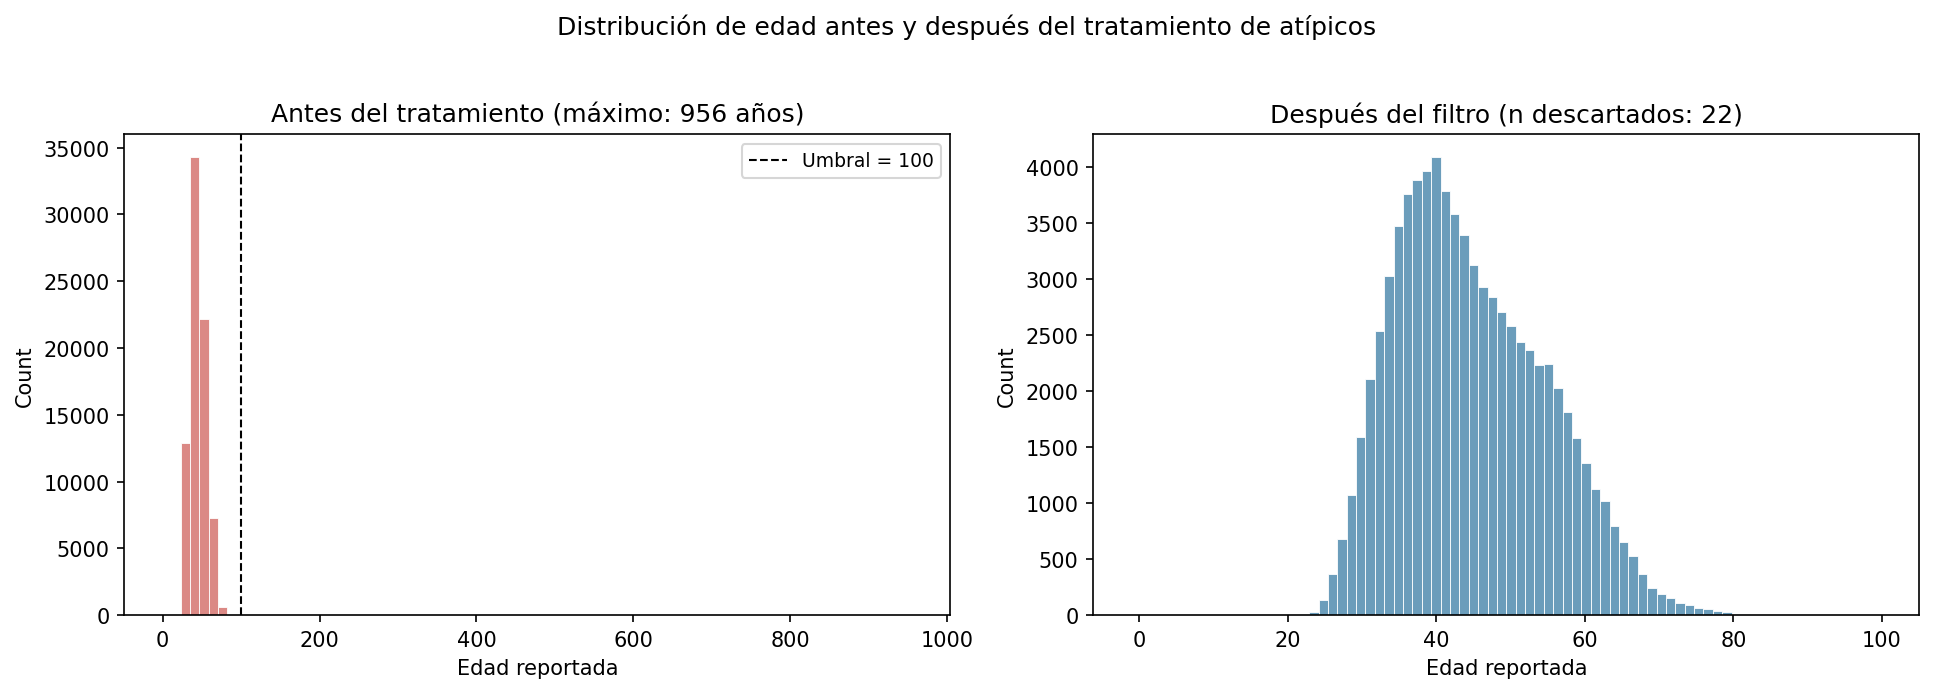
\includegraphics[width=0.92\linewidth]{../../artifacts/sprint6_calidad/fig_edad_antes_despues.png}
\caption{Distribución de edad antes y después del tratamiento de atípicos. El umbral aplicado es 100 años; los 22 casos descartados quedan documentados en \texttt{evidencias/calidad\_atipicos\_edad.csv}.}
\end{figure}

\subsection{Instituciones sin normalizar}\label{ssec:h2}

\begin{hallazgo}
\textbf{Hallazgo 2.} La columna \texttt{inst\_filia} registra \num{2762} entidades únicas; cerca de \num{800} son IES reales. La tabla maestra entregada con este informe (sección \ref{ssec:tabla-maestra}) consolida 211 IES canónicas y cubre el 91\,\% del padrón.
\end{hallazgo}

\begin{figure}[h]
\centering
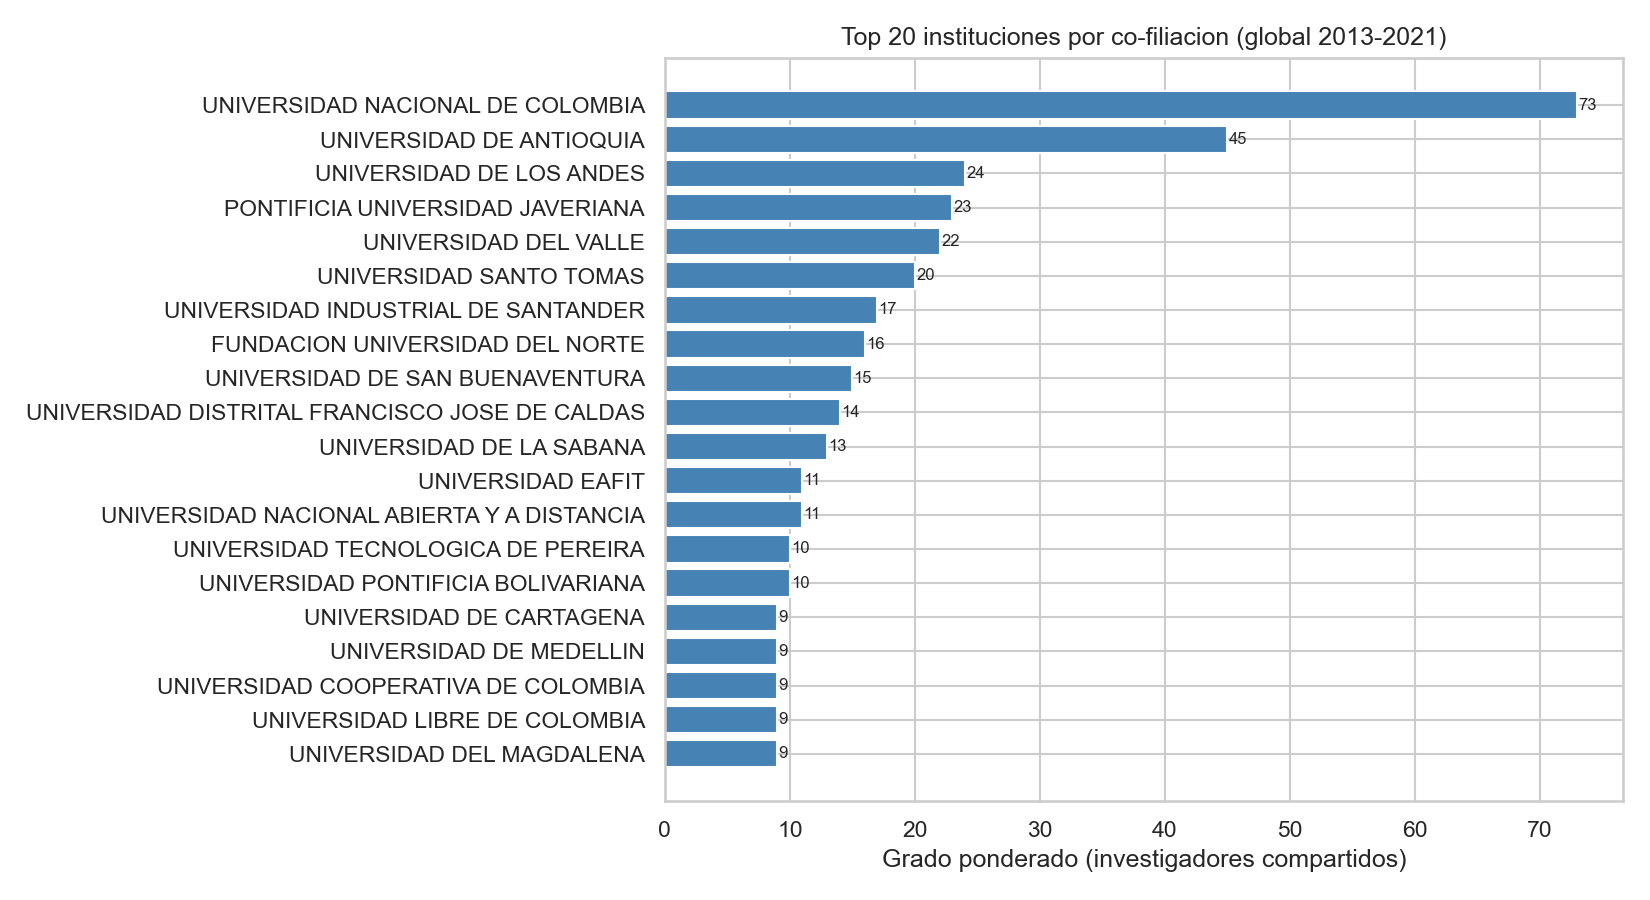
\includegraphics[width=0.95\linewidth]{../../artifacts/sprint3_redes/fig03_top_instituciones.png}
\caption{Top instituciones por número de reconocimientos, después de aplicar la normalización propuesta.}
\end{figure}

El caso prototípico es la Universidad Nacional. Sus cuatro sedes principales --- Bogotá, Medellín, Manizales y Palmira --- aparecen como entidades separadas en el dataset crudo. Cualquier ranking sin tabla maestra infla el número de actores y oculta la concentración real. La tabla maestra que entregamos resuelve estos casos típicos.

\subsection{Diversidad invisible ocho años}\label{ssec:h3-cobertura}

\begin{hallazgo}
\textbf{Hallazgo 3.} Las variables \texttt{ID\_VICTIMA\_CONFLICTO}, \texttt{TXT\_GRUPO\_ETNICO} y \texttt{TXT\_POBLACION\_DISCA} tienen 0\,\% de cobertura en las cinco convocatorias entre 2013 y 2019. Sólo a partir de 2021 se empieza a registrar, con cobertura cercana al 97\,\%.
\end{hallazgo}

\begin{figure}[h]
\centering
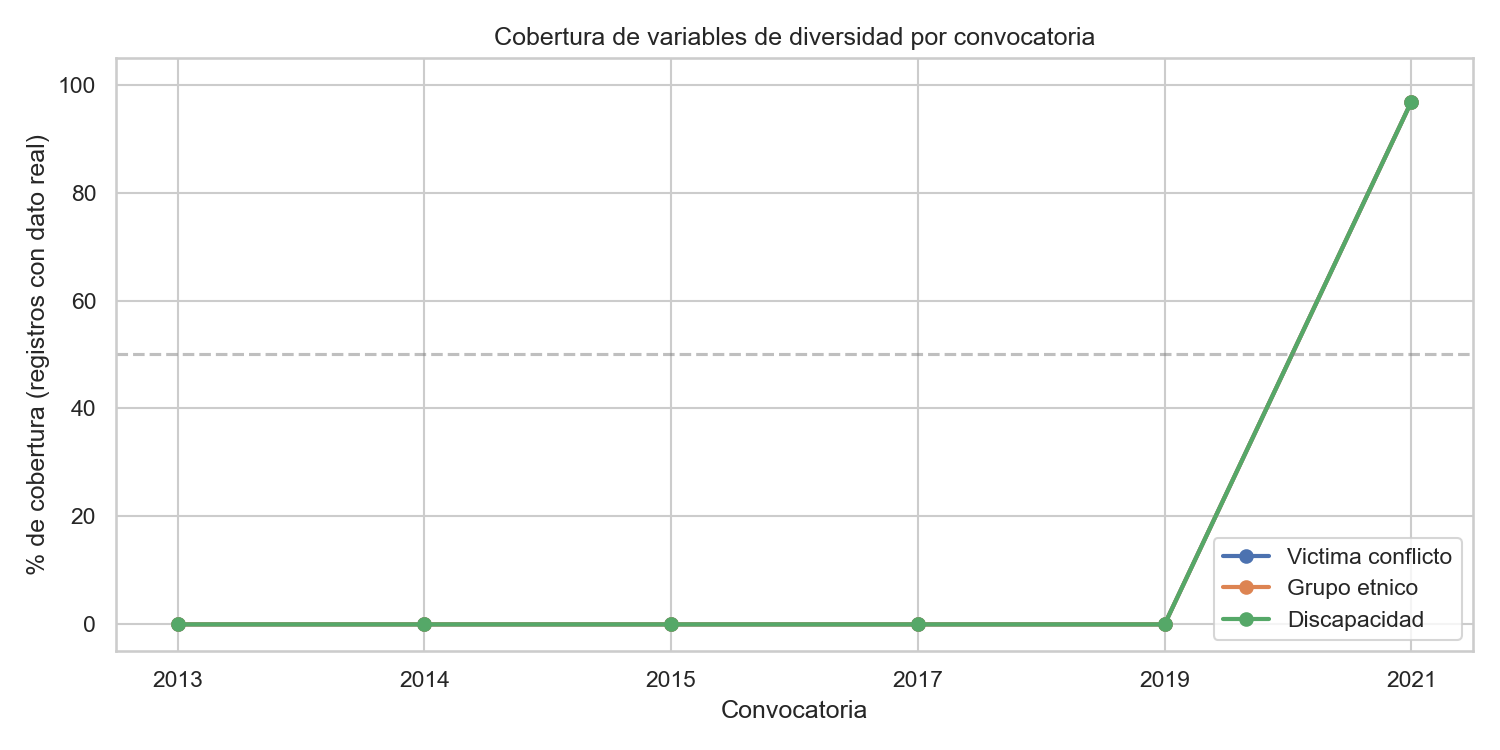
\includegraphics[width=0.95\linewidth]{../../artifacts/sprint4_diversidad/fig01_cobertura_temporal.png}
\caption{Cobertura temporal de las variables de diversidad. En 2013--2019 todos los registros aparecen como ``NO REGISTRA''.}
\end{figure}

Cualquier análisis sobre tendencias en la representación de minorías es estructuralmente imposible. Sólo hay un punto temporal con datos. No es una limitación del análisis: es una restricción heredada del formulario de captura.

\textbf{Sobre retropolación.} Una posibilidad considerada fue asumir que un investigador que en 2021 declaró ser víctima del conflicto ya lo era en 2015, asignando el valor hacia atrás. La idea se descartó porque la condición de víctima del conflicto no es estática --- alguien puede no haberlo sido hace cinco años y serlo hoy --- y el dataset no permite saber la fecha del evento.

% =====================================================================
\section{Trayectoria longitudinal}\label{sec:longitudinal}
% =====================================================================

Reconstruir las seis convocatorias como serie permite preguntar qué le pasa a cada investigador entre una convocatoria y la siguiente.

\subsection{Crecimiento del padrón}

\begin{figure}[h]
\centering
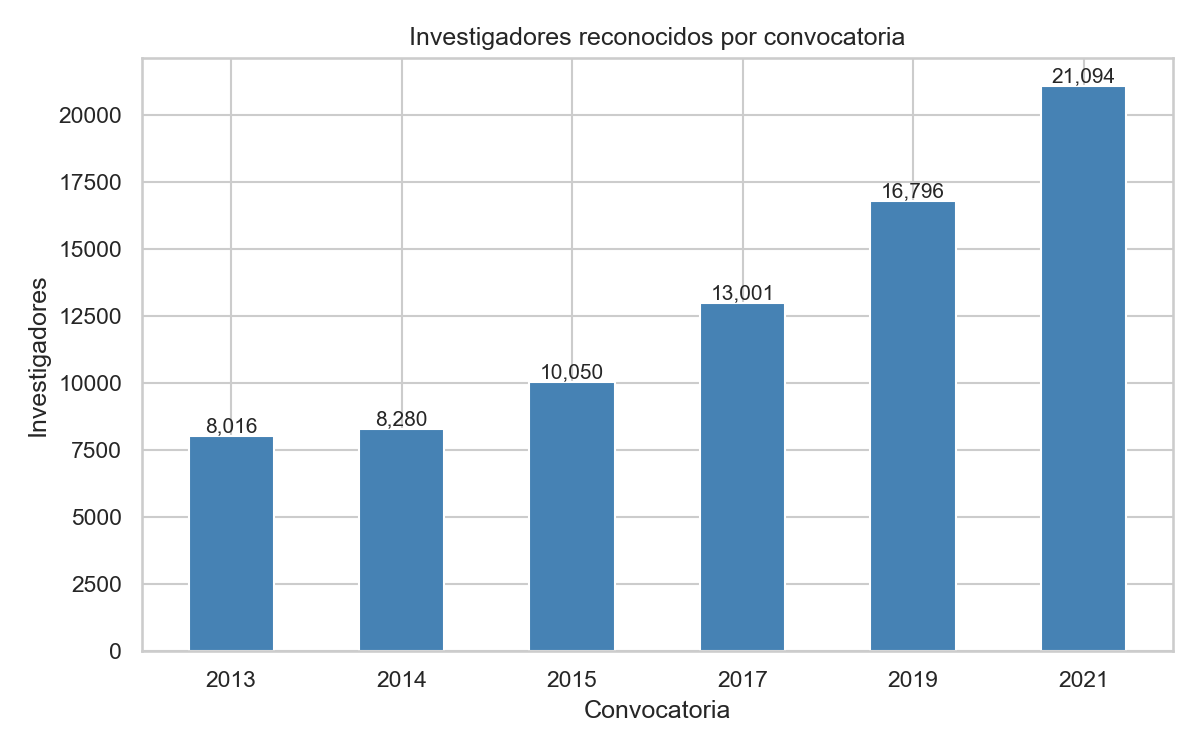
\includegraphics[width=0.9\linewidth]{../../artifacts/sprint2_longitudinal/fig01_evolucion_total.png}
\caption{Evolución del número total de investigadores reconocidos por convocatoria.}
\end{figure}

El padrón pasó de poco más de ocho mil reconocidos en 2013 a más de veintiún mil en 2021. El crecimiento es sostenido pero no uniforme: la convocatoria 2018 representa un salto fuerte respecto a 2017, y 2021 suma otros cinco mil reconocidos. Parte del crecimiento es captura nueva; parte, investigadores que regresan tras una ausencia.

\subsection{Retención y rotación}

\begin{figure}[h]
\centering
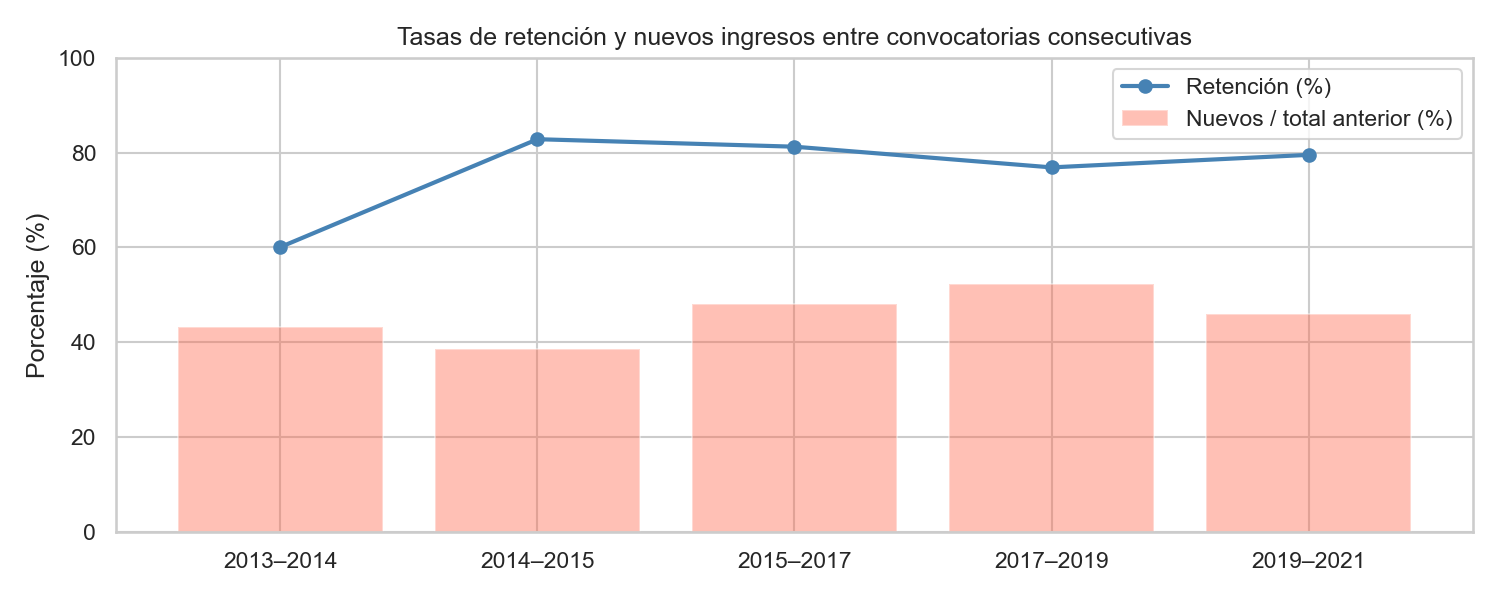
\includegraphics[width=0.9\linewidth]{../../artifacts/sprint2_longitudinal/fig07_retencion.png}
\caption{Tasa de retención entre convocatorias consecutivas.}
\end{figure}

La retención oscila entre 70\,\% y 80\,\%. Parte se explica por requisitos de productividad mínima cuya ventana de evaluación cambia entre convocatorias; parte, por la naturaleza voluntaria del registro.

\paragraph{Caso particular: los Eméritos.}
En las seis convocatorias revisadas ningún investigador Emérito reaparece en la convocatoria siguiente. Cien por ciento de ``desaparición'' aparente. La lectura correcta es la opuesta a lo que sugiere el dato: \textbf{el reconocimiento Emérito queda vitalicio}. No reaparecen porque no necesitan re-postularse. La ausencia en convocatorias posteriores es diseño del sistema, no expulsión.

\subsection{Matrices de transición y Sankeys}

\begin{figure}[h]
\centering
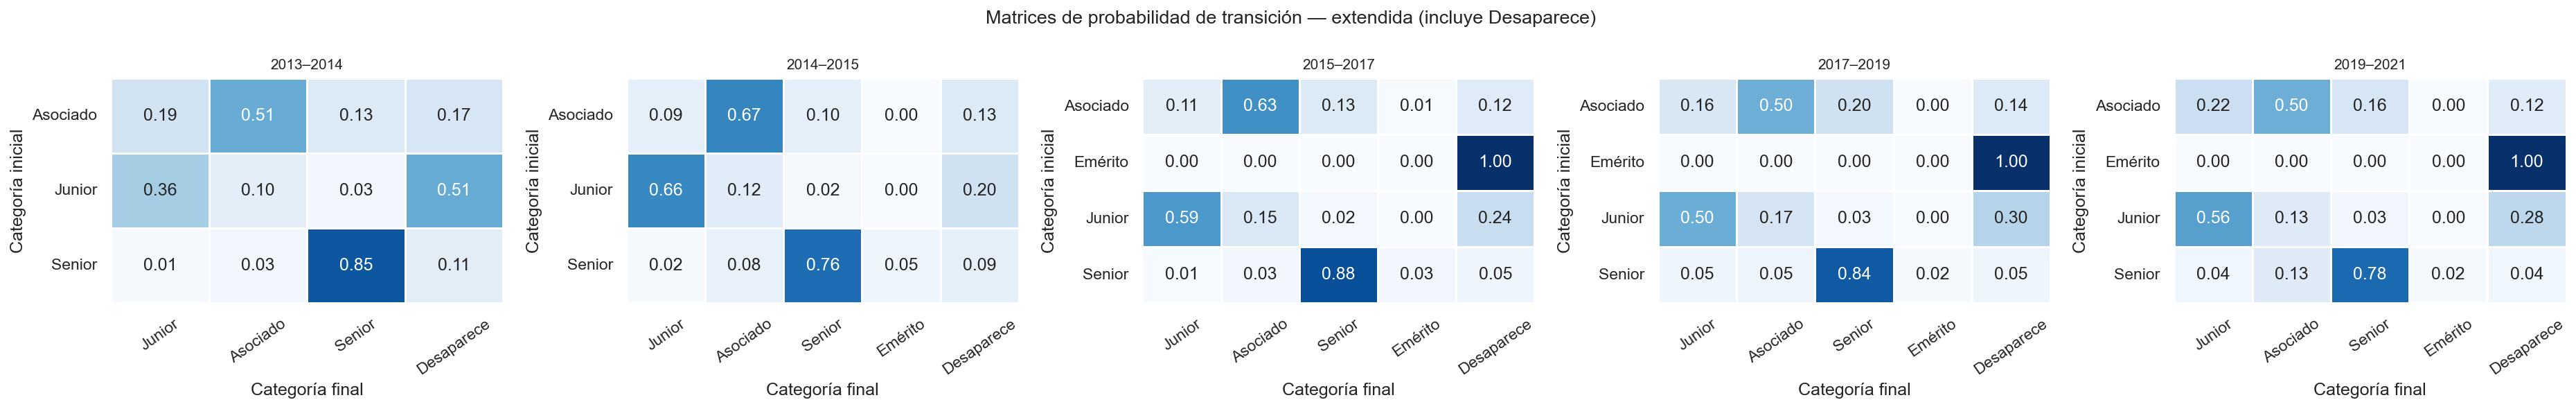
\includegraphics[width=0.95\linewidth]{../../artifacts/sprint2_transiciones/fig01_heatmaps_ext.png}
\caption{Matrices de transición de categorías. Filas: categoría en $t$; columnas: categoría en $t+1$; columna ``Desaparece'' para los que no continúan.}
\end{figure}

\begin{figure}[h]
\centering
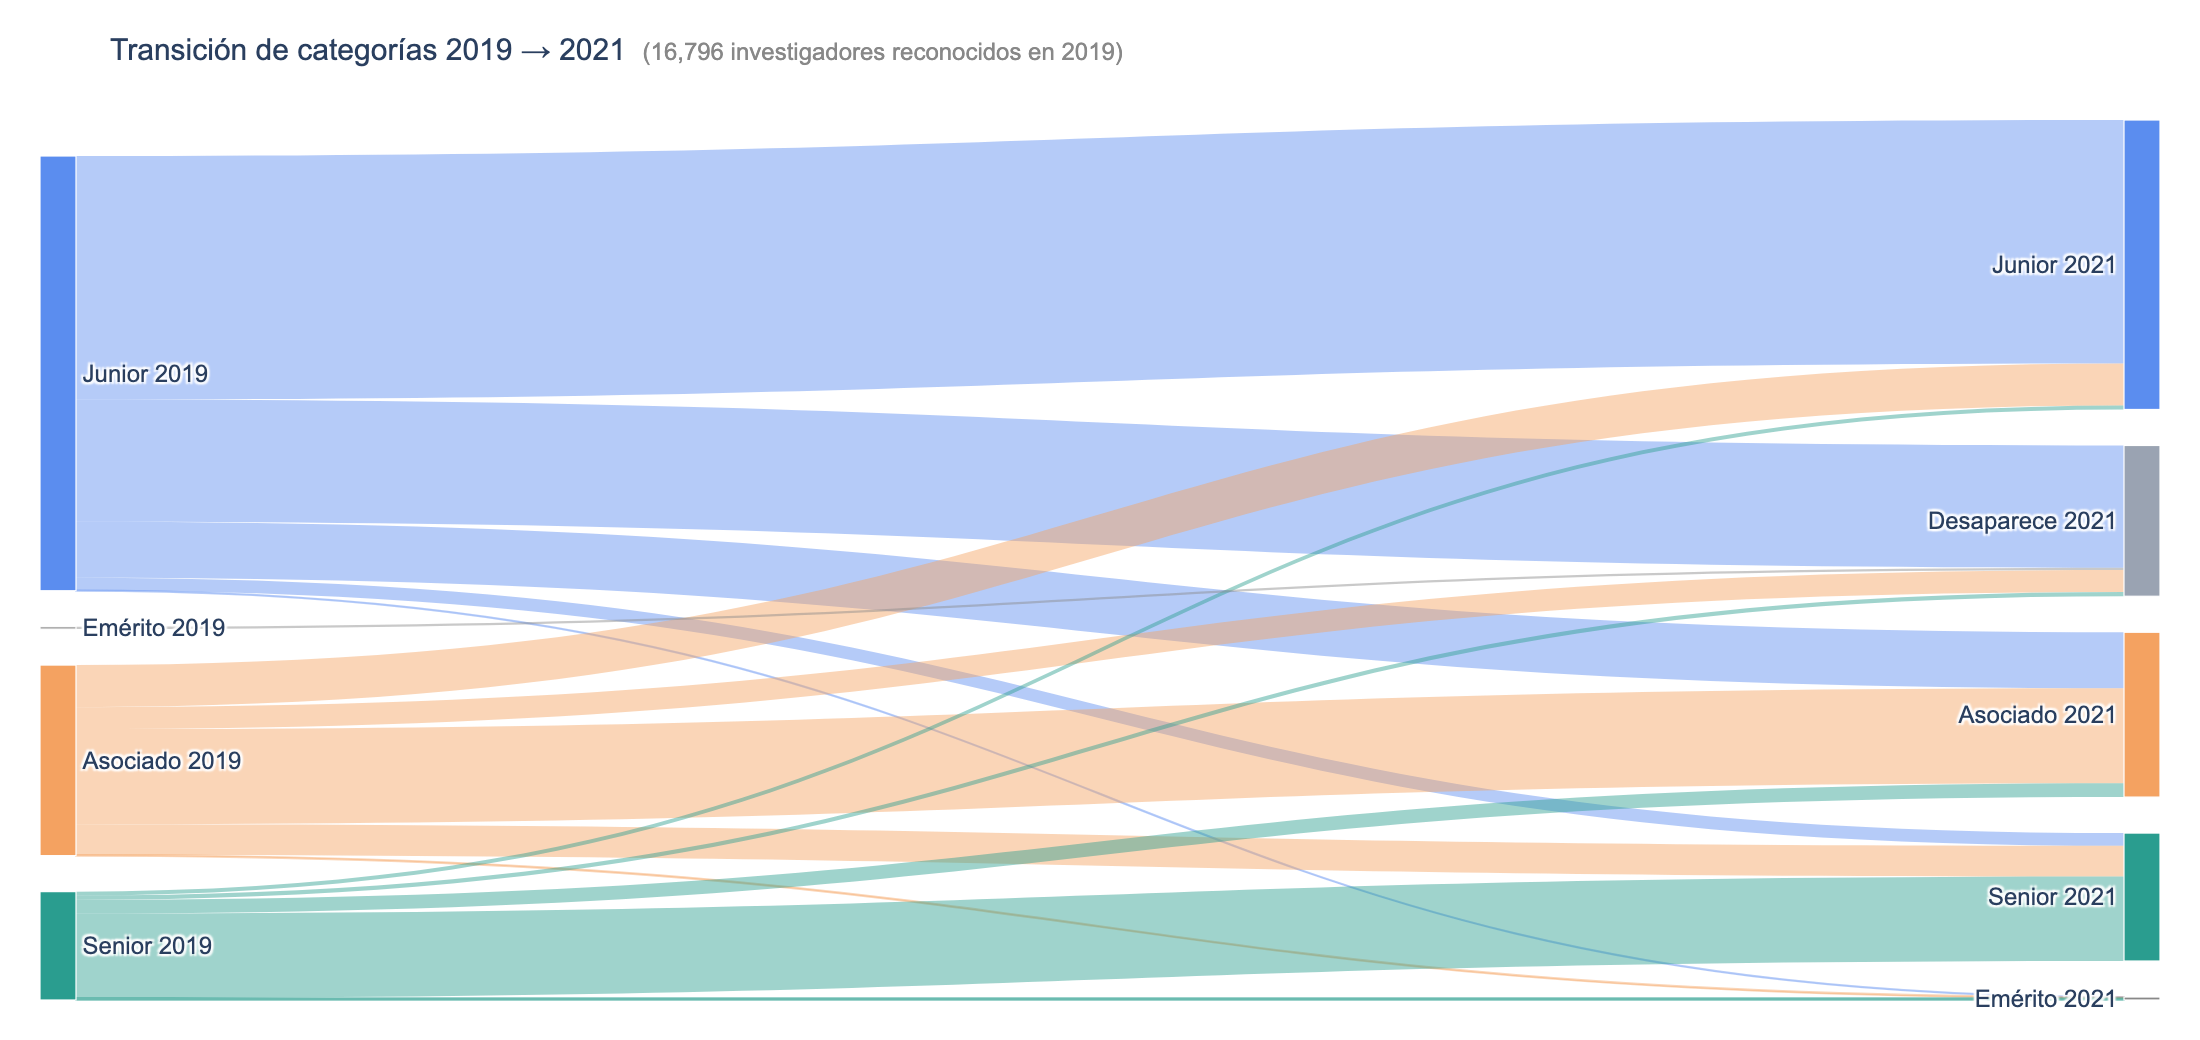
\includegraphics[width=0.95\linewidth]{../../artifacts/sprint6_sankey/sankey_2019_2021.png}
\caption{Sankey de transición de categorías para el último par consecutivo (2019 → 2021). La diagonal principal es permanencia; las bandas hacia arriba son ascensos, las hacia abajo descensos, y la columna ``Desaparece'' agrupa a los que no aparecen en 2021. Para los cuatro pares anteriores ver \texttt{artifacts/sprint6\_sankey/}.}
\end{figure}

\begin{hallazgo}
\textbf{Hallazgo 4.} Las matrices muestran un patrón consistente con la frase del director: ``\textit{la mayoría de Asociados pasaron a Junior porque dejaron de producir}''. Los descensos no son raros y se concentran desde la categoría Asociado. Los ascensos son menos frecuentes que las desapariciones. La ``desaparición'' desde Junior es el flujo más fuerte en cada par consecutivo.
\end{hallazgo}

% =====================================================================
\section{Concentración territorial}\label{sec:territorial}
% =====================================================================

\subsection{Bogotá y Antioquia concentran el 51\,\% del país}\label{ssec:h5}

\begin{hallazgo}
\textbf{Hallazgo 5.} Bogotá D.C.\ representa el 32\,\% del padrón, Antioquia el 16\,\%. Entre las dos suman el 51\,\%. El restante 49\,\% se distribuye entre los otros 30 departamentos. Veintidós departamentos no llegan a 500 investigadores reconocidos.
\end{hallazgo}

\begin{figure}[h]
\centering
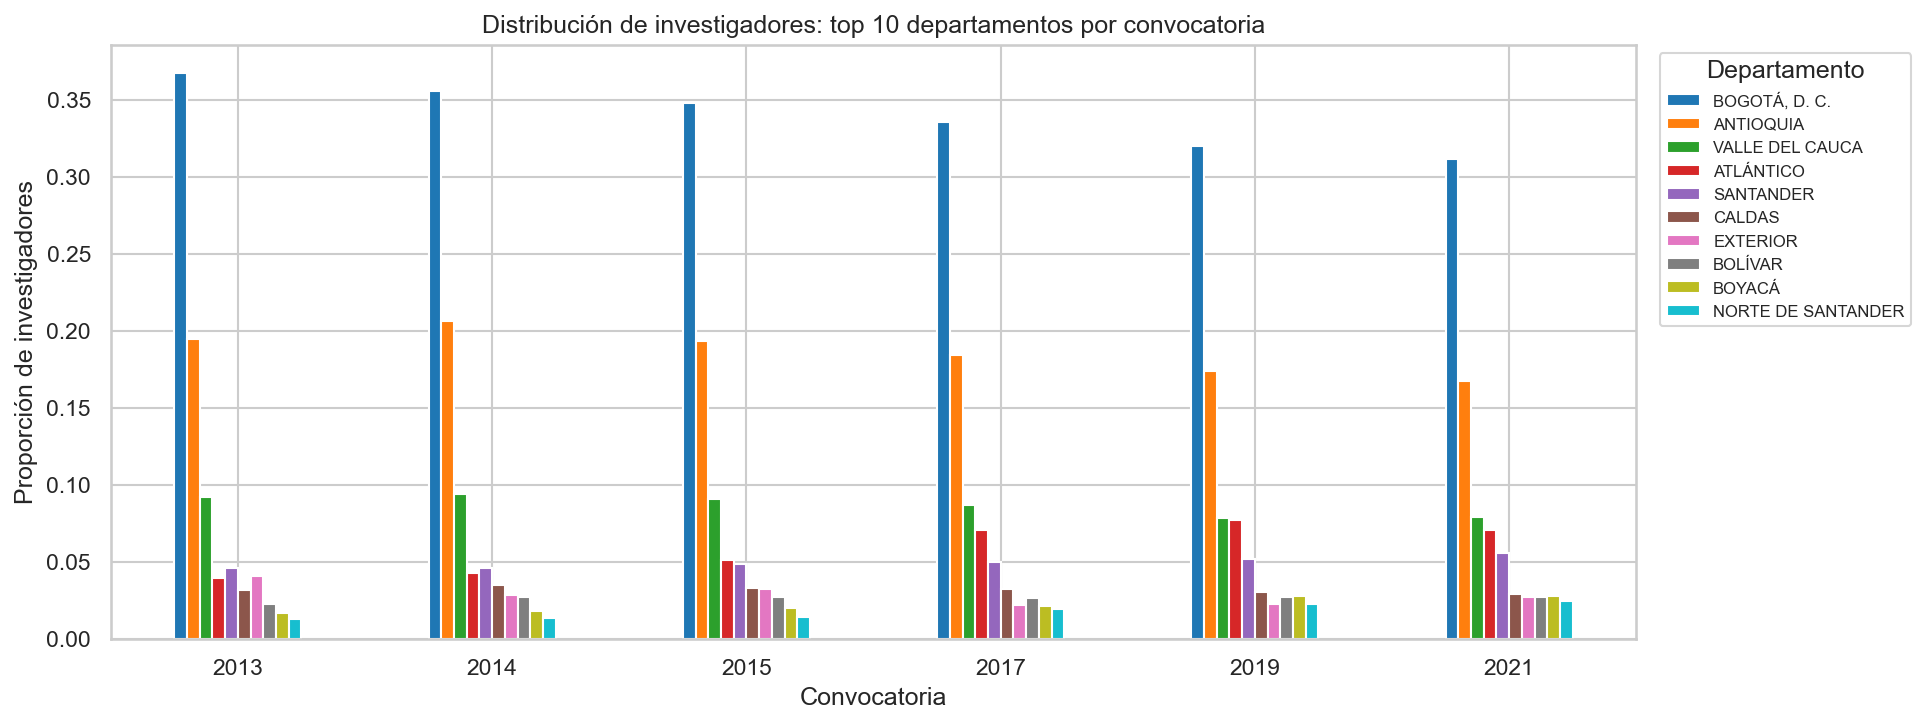
\includegraphics[width=0.95\linewidth]{../../artifacts/sprint2_territorial/fig01_top_departamentos.png}
\caption{Distribución de investigadores reconocidos por departamento de residencia (acumulado de las seis convocatorias).}
\end{figure}

La evolución del HHI por convocatoria confirma que la concentración no se ha reducido sustancialmente en la década. Si las políticas de descentralización del conocimiento están operando, su efecto no es perceptible en este indicador.

\subsection{Productividad por territorio}\label{ssec:h6}

\begin{hallazgo}
\textbf{Hallazgo 6.} El ratio entre porcentaje de productos y porcentaje de investigadores muestra que algunas regiones medianas son más productivas por capita que las grandes. Bolívar y Risaralda alcanzan ratios de 1{,}24. Los investigadores con residencia en el exterior caen a 0{,}34.
\end{hallazgo}

\begin{figure}[h]
\centering
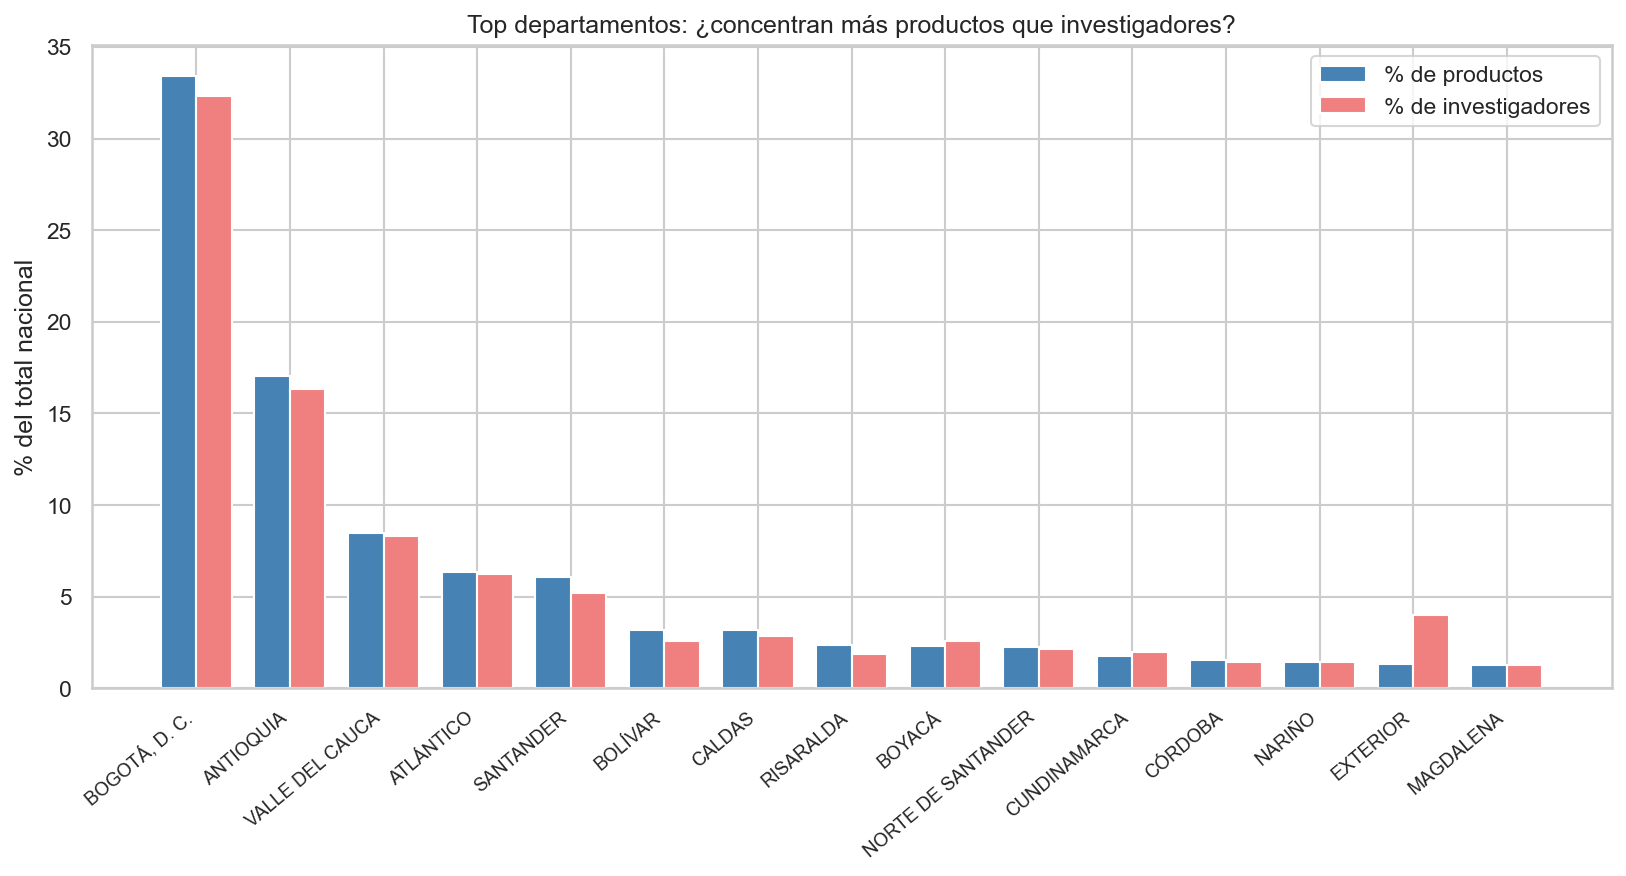
\includegraphics[width=0.92\linewidth]{../../artifacts/sprint5_produccion/fig04_concentracion_territorial.png}
\caption{Top quince departamentos: porcentaje de productos vs.\ porcentaje de investigadores reconocidos.}
\end{figure}

Bogotá y Antioquia tienen ratios cercanos a 1: producen lo que su peso en el padrón sugiere. Bolívar y Risaralda producen más por investigador. La centralización del padrón no se traduce en centralización de la productividad: las regiones medianas tienen efectos por encima de su tamaño.

\subsection{¿Dónde reside el investigador y dónde trabaja?}\label{ssec:h7-geografia}

Con la tabla maestra de instituciones podemos preguntar algo que el dataset por sí solo no permite: dónde trabaja el investigador, no sólo dónde reside. El cruce \texttt{departamento de residencia} × \texttt{departamento de la sede institucional} produce los flujos que aparecen en la figura \ref{fig:heatmap-geog}.

\begin{figure}[h]
\centering
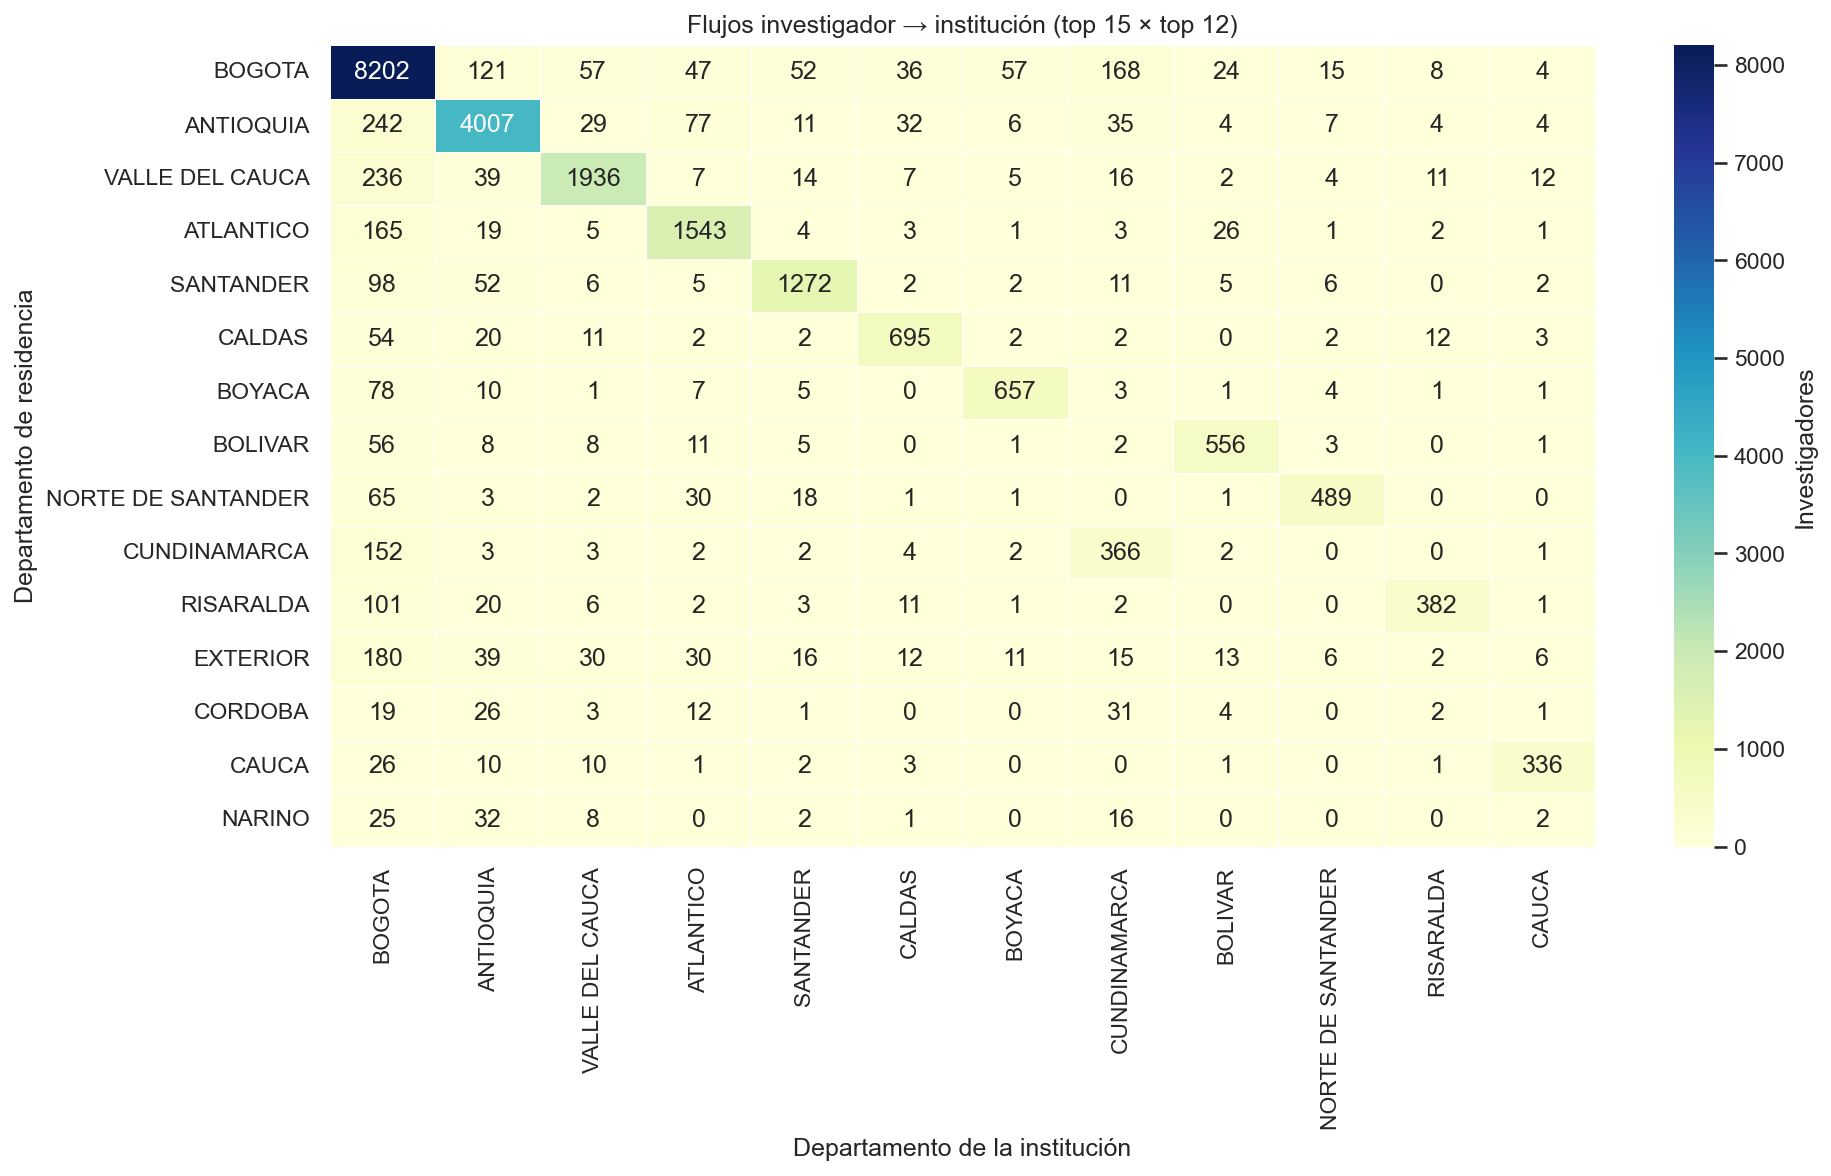
\includegraphics[width=0.95\linewidth]{../../artifacts/sprint6_geografia/fig_heatmap_residencia_institucion.png}
\caption{Flujos residencia → institución (top 15 departamentos × top 12 destinos). Las celdas muestran el número de investigadores únicos en cada par.}
\label{fig:heatmap-geog}
\end{figure}

\begin{hallazgo}
\textbf{Hallazgo 7.} Bogotá no sólo concentra (32\,\% del padrón) sino que \textbf{atrae} investigadores que residen en otros departamentos. El flujo transversal más fuerte es Antioquia → Bogotá (242 investigadores), seguido de Valle del Cauca → Bogotá (236) y Exterior → Bogotá (180). El movimiento inverso es menor.
\end{hallazgo}

\begin{table}[h]
\centering
\caption{Retención local por departamento de residencia (\% de investigadores que trabajan en su mismo departamento).}
\label{tab:retencion-local}
\small
\begin{tabular}{l r r l}
\toprule
\textbf{Departamento} & \textbf{N} & \textbf{\% local} & \textbf{Destino externo principal} \\
\midrule
Bogotá D.C.        & 8.934 & 92\,\% & Cundinamarca (168) \\
Antioquia          & 4.490 & 89\,\% & Bogotá (242) \\
Atlántico          & 1.804 & 86\,\% & Bogotá (165) \\
Santander          & 1.482 & 86\,\% & Bogotá (98) \\
Boyacá             &   772 & 85\,\% & Bogotá (78) \\
Risaralda          &   541 & 71\,\% & Bogotá (101) \\
Cundinamarca       &   548 & 67\,\% & Bogotá (152) \\
Chocó              &    49 & 92\,\% & Valle del Cauca (2) \\
Amazonas           &    34 & 76\,\% & Bogotá (5) \\
Vichada            &     1 &  0\,\% & Bogotá (1) \\
\bottomrule
\end{tabular}
\end{table}

\begin{figure}[h]
\centering
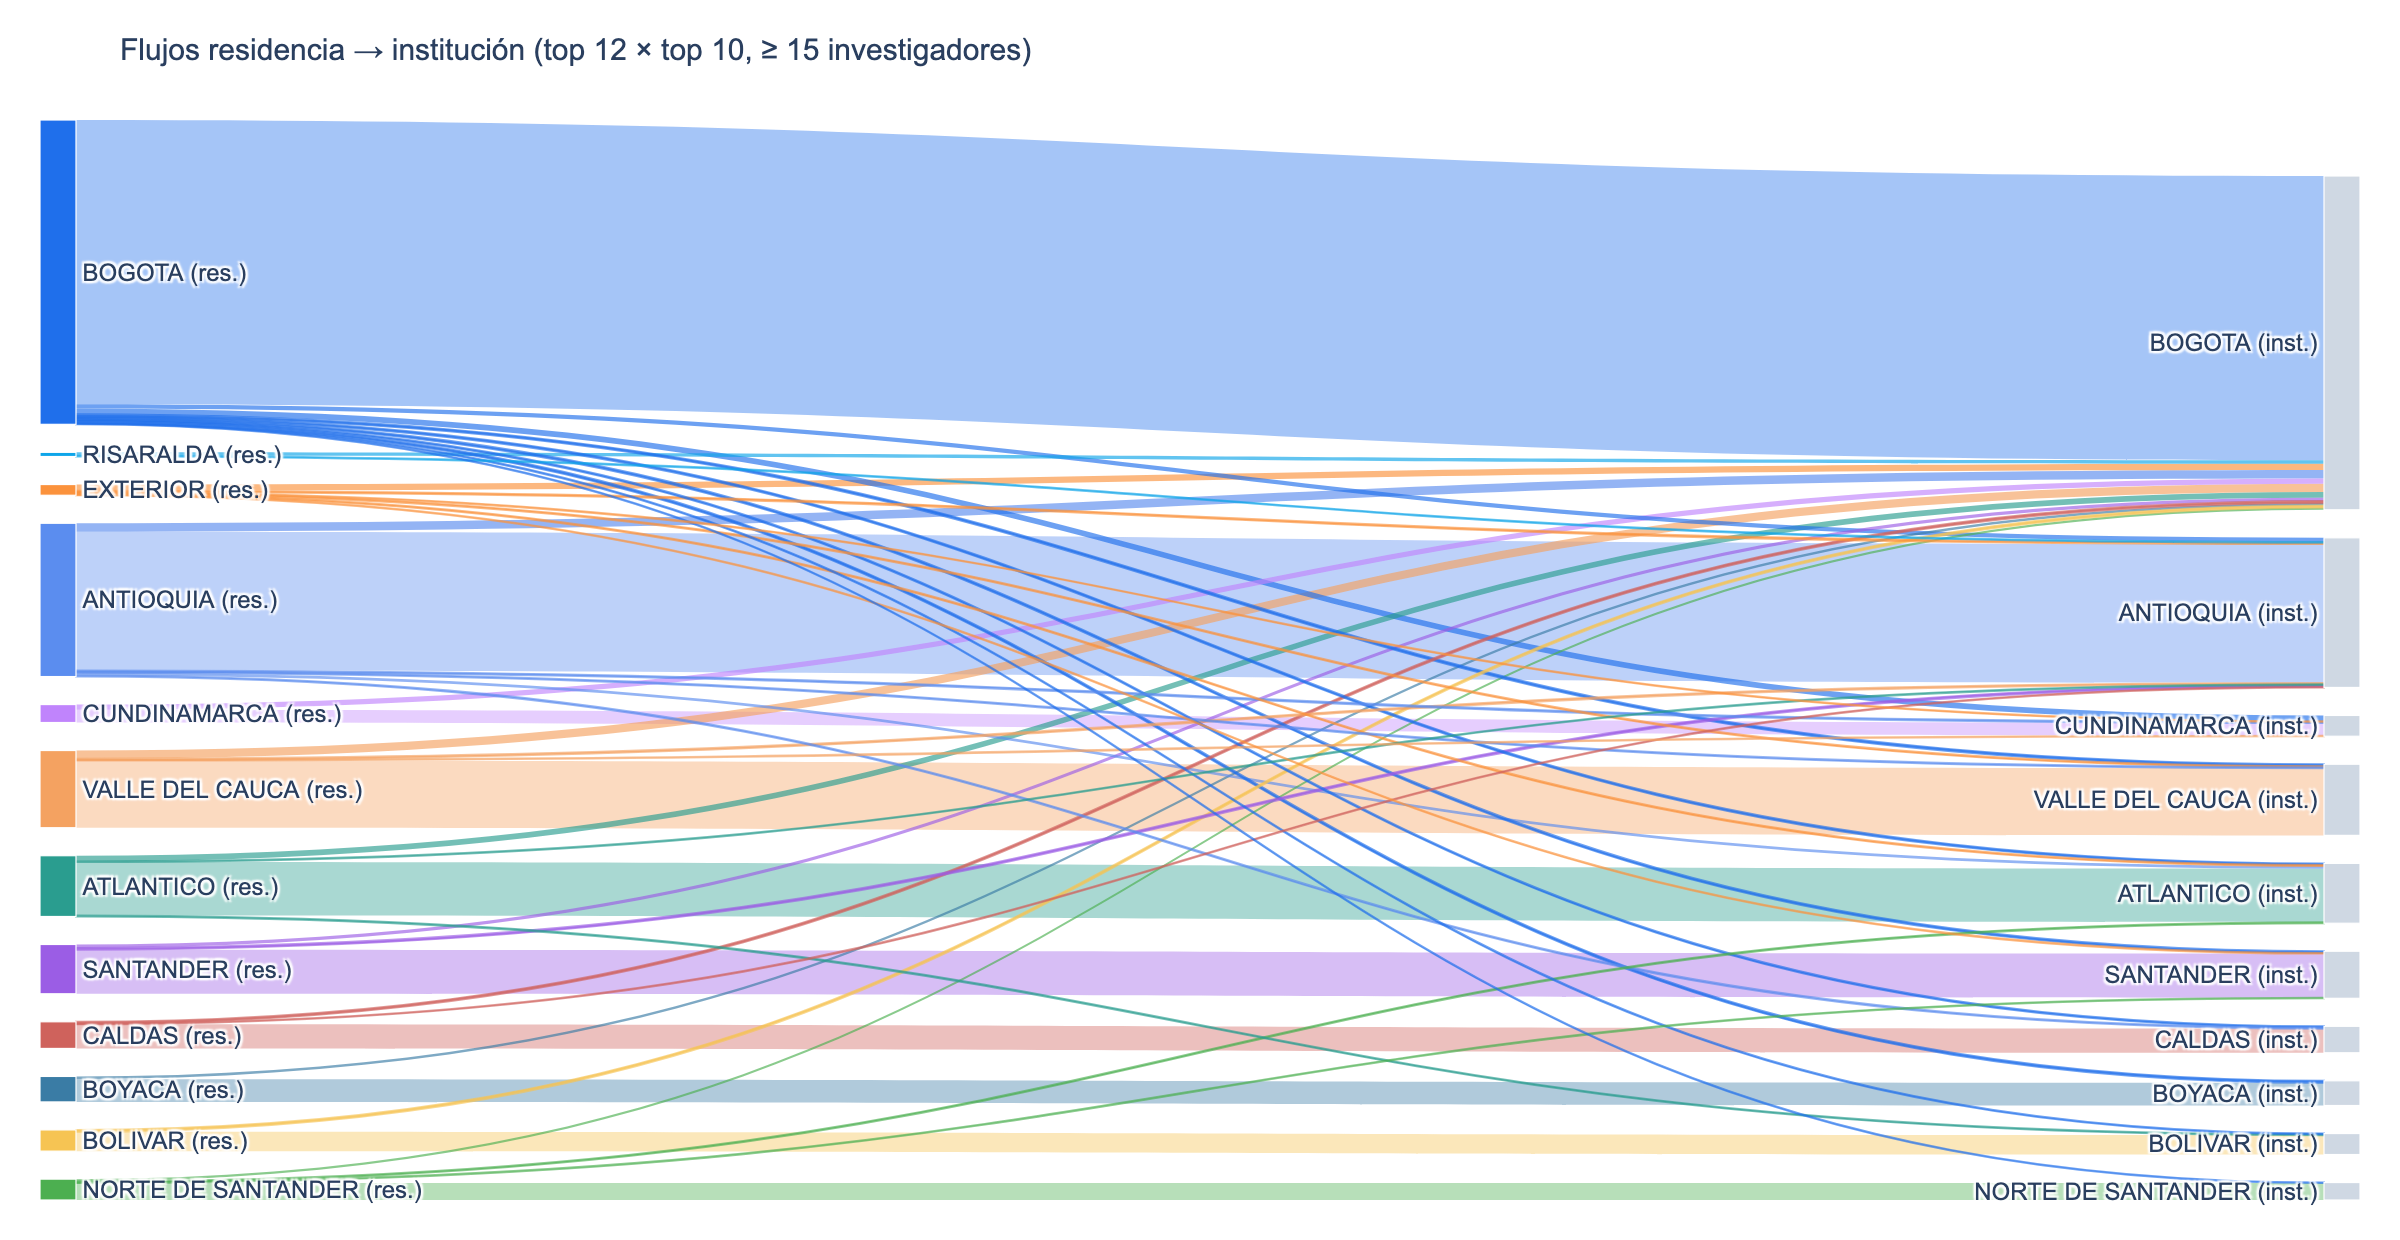
\includegraphics[width=0.9\linewidth]{../../artifacts/sprint6_sankey/sankey_territorial.png}
\caption{Sankey territorial: flujos residencia → departamento institucional. Top doce departamentos por volumen, flujos $\geq$ 15 investigadores.}
\end{figure}

Dos lecturas se desprenden:

\begin{enumerate}[label=(\alph*),leftmargin=*]
\item \textbf{Bogotá no sólo concentra: absorbe.} Investigadores de prácticamente todos los demás departamentos terminan afiliados a instituciones bogotanas. Cundinamarca, departamento limítrofe, registra el 67\,\% de retención local: un tercio de sus investigadores trabaja en Bogotá.
\item \textbf{Las regiones periféricas muestran patrones distintos.} Chocó sostiene una retención local del 92\,\% pese a tener apenas 49 investigadores reconocidos; Amazonas, del 76\,\%; el único caso de Vichada se va para Bogotá. Es decir, donde hay instituciones funcionales con investigadores reconocidos, la retención local es alta independientemente del tamaño del padrón.
\end{enumerate}

% =====================================================================
\section{Brecha de género}\label{sec:genero}
% =====================================================================

\subsection{Representación femenina por área}\label{ssec:h8}

\begin{hallazgo}
\textbf{Hallazgo 8.} La participación femenina en el padrón es de aproximadamente 40\,\% global. El promedio oculta brechas estructurales por gran área OCDE: 24\,\% en Ingeniería y Tecnología, 48\,\% en Ciencias Médicas, cerca de la paridad en Humanidades y Ciencias Sociales.
\end{hallazgo}

\begin{figure}[h]
\centering
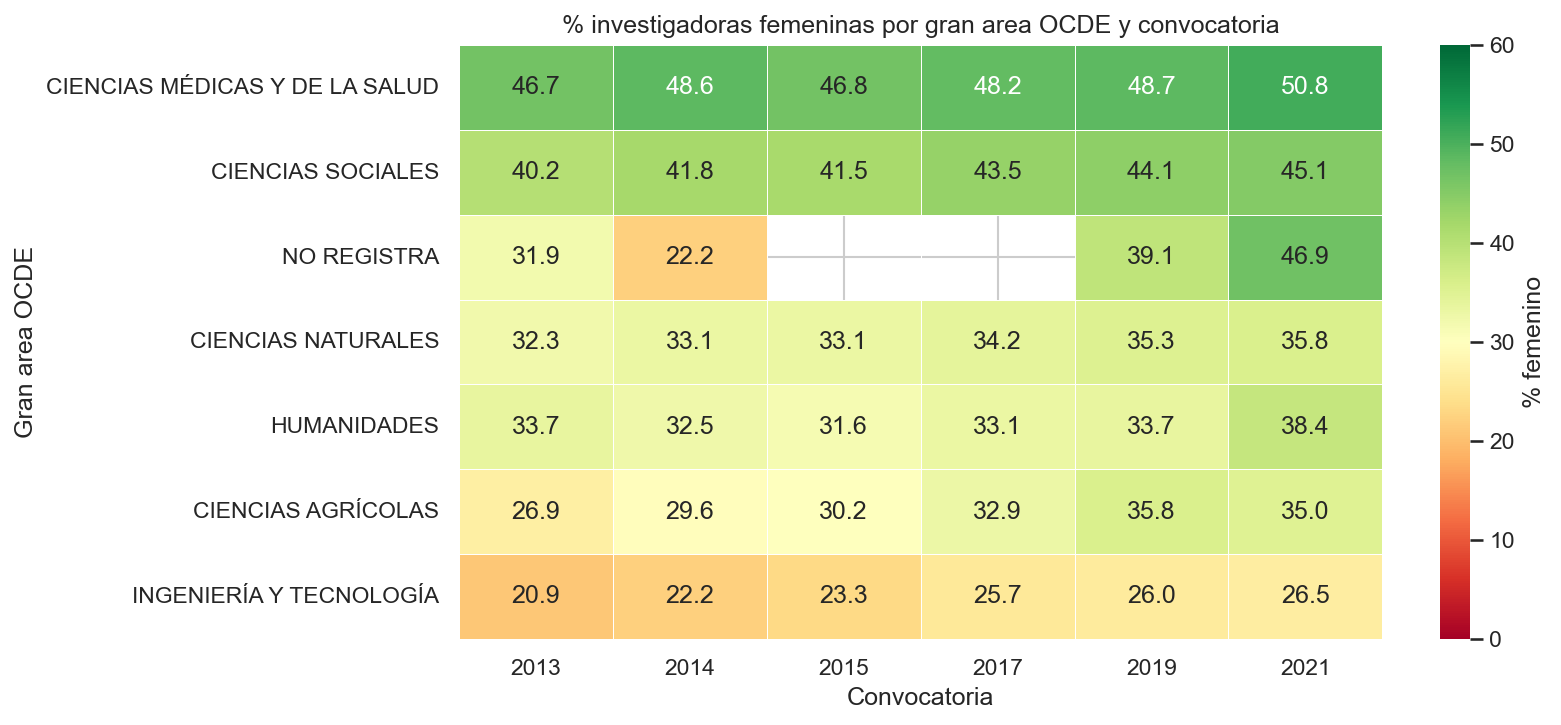
\includegraphics[width=0.95\linewidth]{../../artifacts/sprint2_genero_ocde/fig02_heatmap_pct_femenino.png}
\caption{Porcentaje de mujeres por gran área OCDE y convocatoria.}
\end{figure}

La cifra agregada de 40\,\% genera una sensación de cercanía a la paridad que no se sostiene por área. Las disciplinas STEM mantienen una sub-representación femenina que no se ha movido durante la década observada.

\subsection{Brecha en productividad}\label{ssec:h9}

\begin{hallazgo}
\textbf{Hallazgo 9.} Una vez dentro del sistema, las mujeres registran menos productos en promedio que los hombres en cinco de las seis grandes áreas. La única excepción es Humanidades. Mayores brechas: Ciencias Médicas (--2{,}95 productos) e Ingeniería (--2{,}59).
\end{hallazgo}

\begin{figure}[h]
\centering
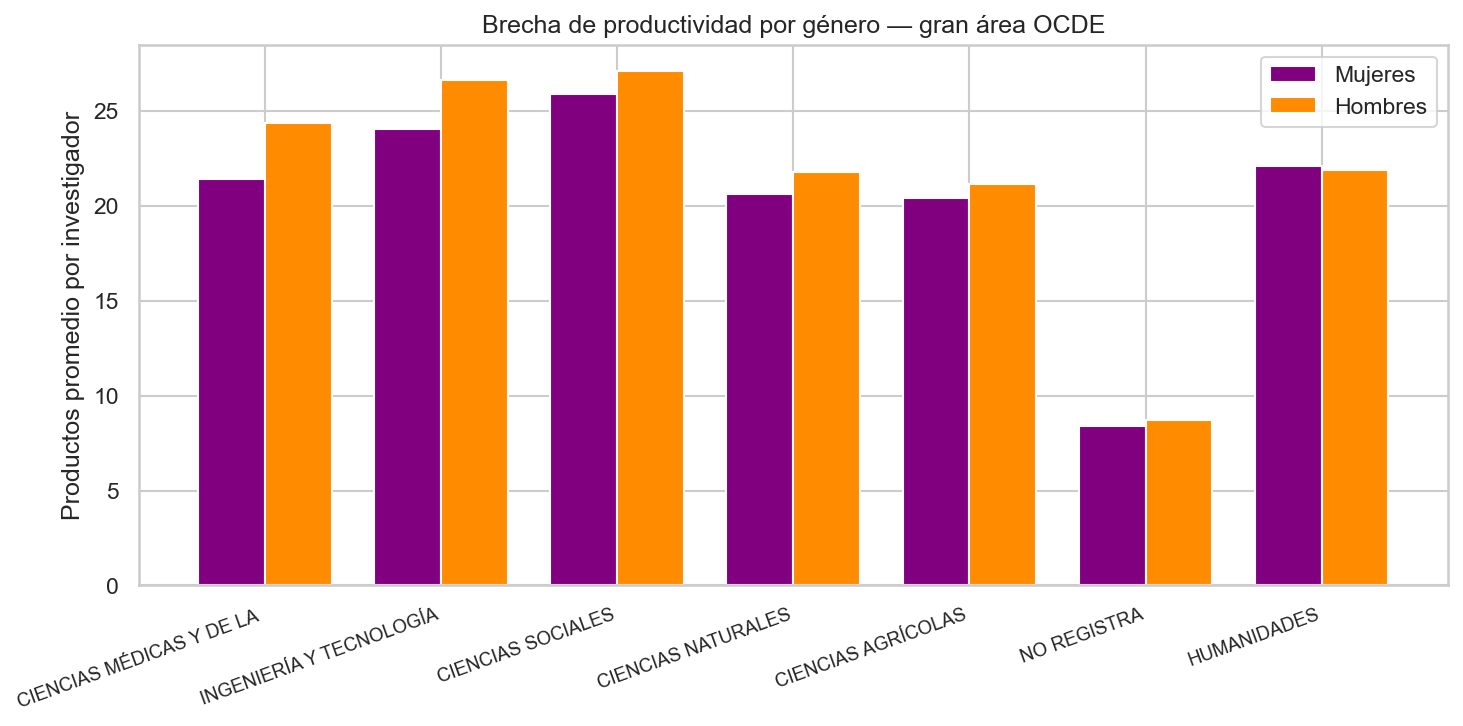
\includegraphics[width=0.95\linewidth]{../../artifacts/sprint5_produccion/fig03_brecha_genero_productividad.png}
\caption{Brecha de productividad por género en cada gran área OCDE.}
\end{figure}

Pocas mujeres entran al sistema, y a las que entran se les contabiliza menos producción. La razón no se reduce a un factor único: pueden estar pesando la distribución de carga académica, la segmentación por tipo de producto, o el efecto de cohorte (las mujeres son en promedio más jóvenes en el padrón). El dato es que la métrica oficial de productividad no se desempaña por género.

% =====================================================================
\section{Diversidad: étnia, discapacidad, conflicto}\label{sec:diversidad}
% =====================================================================

Como se mencionó en \ref{ssec:h3-cobertura}, las variables de diversidad sólo empiezan a registrarse en 2021. Cualquier análisis está limitado a esa convocatoria.

\subsection{Sub y sobre-representación frente a la población}\label{ssec:h10}

\begin{hallazgo}
\textbf{Hallazgo 10.} Comparados con DANE-CNPV 2018 y RUV 2021, los investigadores reconocidos en 2021 muestran subrepresentación significativa de afrocolombianos (3$\times$), indígenas (7,9$\times$), personas con discapacidad (8$\times$) y víctimas del conflicto (8,6$\times$). Por el contrario, raizales, palenqueros y rrom aparecen sobre-representados entre 3$\times$ y 6$\times$.
\end{hallazgo}

\begin{figure}[h]
\centering
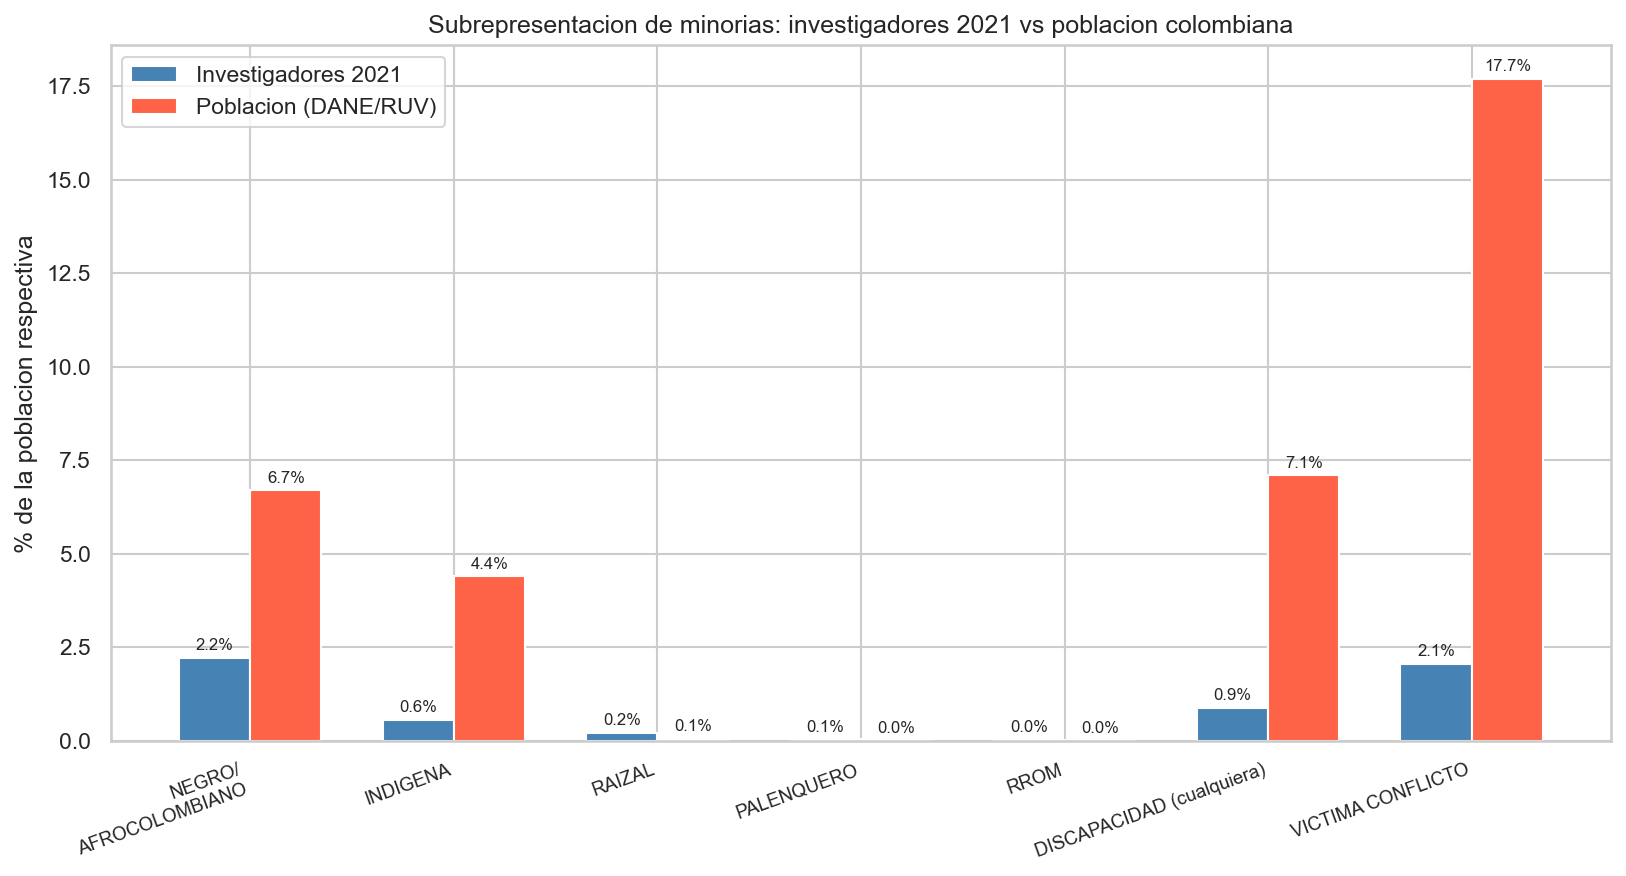
\includegraphics[width=0.95\linewidth]{../../artifacts/sprint4_diversidad/fig02_comparacion_dane.png}
\caption{Composición de los investigadores reconocidos en 2021 vs.\ proporciones poblacionales nacionales.}
\end{figure}

\begin{caveat}
La comparación correcta sería contra la población \emph{con educación superior}, no contra la población total. La participación étnica entre quienes acceden a estudios universitarios ya está sesgada respecto a la composición nacional. La brecha real es probablemente menor a la mostrada en esta figura, sin que eso anule el patrón.
\end{caveat}

% =====================================================================
\section{Redes y poder institucional}\label{sec:redes}
% =====================================================================

\subsection{Co-filiación: artefacto de captura}

\begin{hallazgo}
\textbf{Hallazgo 11.} La doble afiliación institucional sólo aparece registrada en la convocatoria 2019 (833). Cuando un investigador está afiliado a más de una institución, en las convocatorias 2013--2017 y 2021 sólo se registra una de ellas. En 2019 aparecen 569 investigadores con doble afiliación.
\end{hallazgo}

El cambio de cero a 569 registros entre la convocatoria 2017 y la 2019 \emph{no} refleja un cambio en la realidad académica. Refleja un cambio en cómo se captura la información en el formulario de inscripción. Cualquier análisis de redes de colaboración construido sobre este dataset hereda la limitación.

% =====================================================================
\section{Productividad y reconocimiento}\label{sec:productividad}
% =====================================================================

\subsection{Producción y categoría}\label{ssec:h12-cat}

\begin{hallazgo}
\textbf{Hallazgo 12.} La productividad media escala con la categoría reconocida. Junior 30 productos, Asociado 65, \textbf{Senior 121}, Emérito 34.
\end{hallazgo}

\begin{figure}[h]
\centering
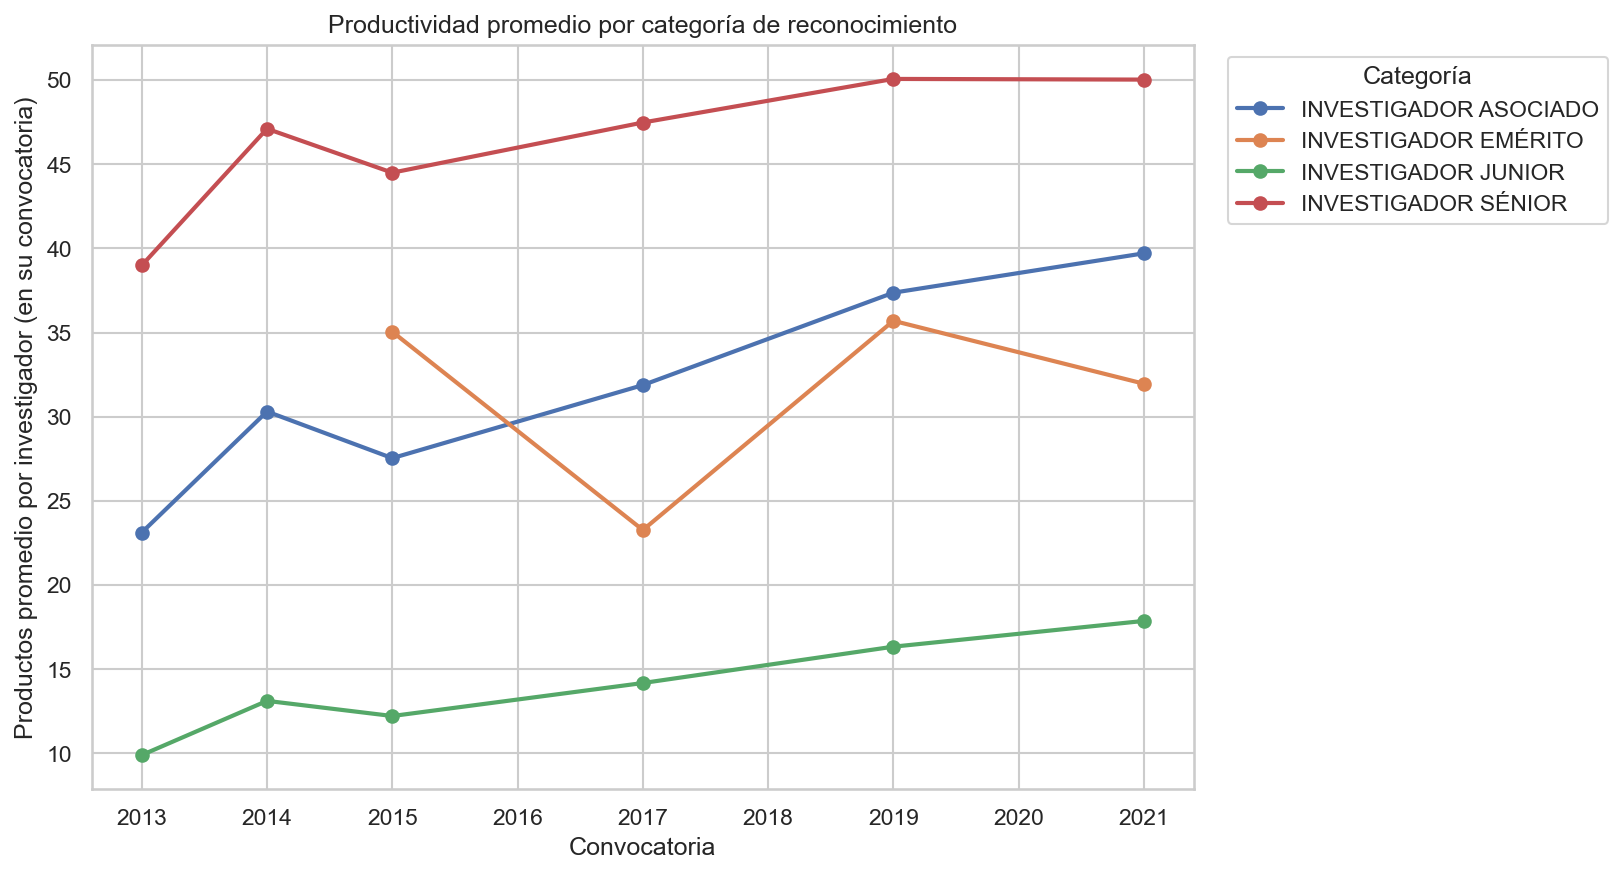
\includegraphics[width=0.95\linewidth]{../../artifacts/sprint5_produccion/fig02_productividad_por_categoria.png}
\caption{Productividad media por categoría a lo largo de las convocatorias 2013--2021.}
\end{figure}

El orden Junior $<$ Asociado $<$ Senior es consistente con el diseño del sistema. Un Senior produce aproximadamente cuatro veces los productos de un Junior. El sistema premia productividad de manera ordenada.

\paragraph{Eméritos.} Los Eméritos producen menos que los Asociados (34 vs.\ 65). La cifra no tiene una sola lectura: por un lado, son la categoría más exigente y el corte para entrar es alto; por otro, una vez reconocidos como Eméritos quedan vitalicios y no necesitan acumular más producción. Lo que el dato no captura es lo que producen después del reconocimiento --- que existe, pero no entra a la métrica oficial porque no se postulan otra vez.

\subsection{Composición por gran área OCDE}\label{ssec:ocde-comp}

\begin{hallazgo}
\textbf{Hallazgo 13.} En volumen total, Ciencias Sociales es la rama que más produce (585 mil productos). Pero en productos por investigador domina \textbf{Ingeniería y Tecnología} (67 productos/investigador). Humanidades es la menos productiva por investigador (48).
\end{hallazgo}

\begin{table}[h]
\centering
\caption{Producción por gran área OCDE.}
\small
\begin{tabular}{l r r r}
\toprule
\textbf{Gran área OCDE} & \textbf{N productos} & \textbf{N investigadores} & \textbf{Productos/inv.} \\
\midrule
Ciencias Sociales              & 585.143 & 9.386 & 62 \\
Ingeniería y Tecnología        & 388.389 & 5.788 & \textbf{67} \\
Ciencias Naturales             & 386.674 & 6.641 & 58 \\
Ciencias Médicas y de la Salud & 275.346 & 4.684 & 59 \\
Humanidades                    & 120.059 & 2.511 & 48 \\
Ciencias Agrícolas             &  75.685 & 1.440 & 53 \\
\bottomrule
\end{tabular}
\end{table}

La diferencia entre volumen total y productividad por investigador es importante. Ciencias Sociales es el área más numerosa y por eso produce más en agregado; Ingeniería es más densa por investigador. Esta distinción matiza cualquier afirmación sobre ``qué área produce más en Colombia''.

\subsection{Autoría sin reconocimiento}\label{ssec:h14}

\begin{hallazgo}
\textbf{Hallazgo 14.} El dataset de producción contiene \num{77401} autores únicos. De ellos, \num{28590} están en el padrón de investigadores reconocidos. Los \num{48811} restantes --- el 36{,}9\,\% del total --- firman productos contabilizados por MinCiencias sin estar en el padrón.
\end{hallazgo}

\begin{figure}[h]
\centering
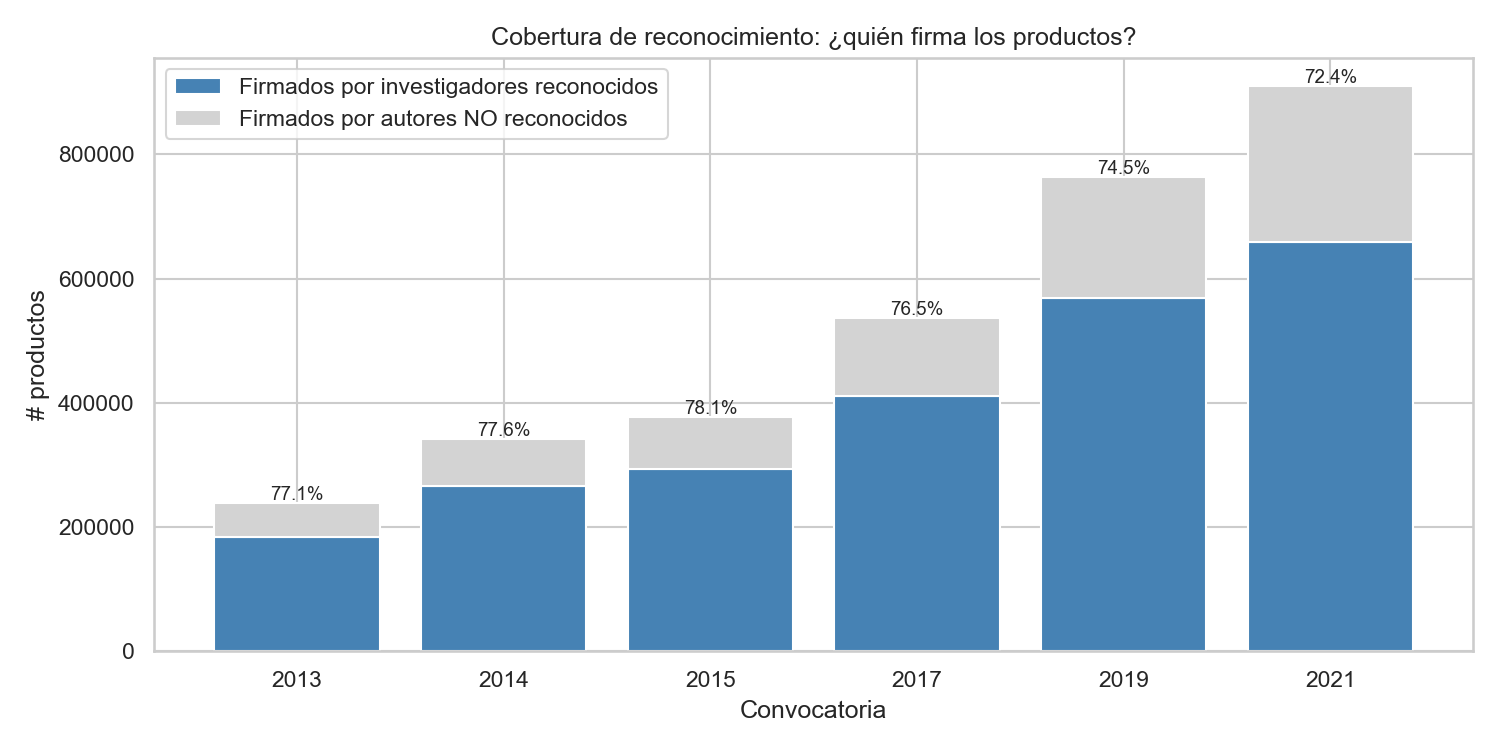
\includegraphics[width=0.95\linewidth]{../../artifacts/sprint5_produccion/fig01_cobertura_reconocidos.png}
\caption{Cobertura de reconocimiento entre los autores de los productos contabilizados, por convocatoria.}
\end{figure}

La proporción de productos firmados por reconocidos pasa del 77\,\% en 2013 al 72\,\% en 2021 --- la coautoría externa al sistema crece. ¿Quiénes son los \num{48811}? El dataset no tiene información biográfica sobre ellos, lo que en sí mismo es revelador: el sistema MinCiencias contabiliza su producción para evaluar grupos pero no los visibiliza individualmente.

Hipótesis sobre quiénes son:

\begin{itemize}
\item Estudiantes de pregrado, maestría o doctorado que coautoran con sus directores.
\item Investigadores extranjeros sin perfil ScienTI que coautoran con colegas colombianos.
\item Profesionales del sector público o privado que participan en proyectos sin formalizar perfil académico.
\item Investigadores colombianos que cumplen requisitos pero no se postulan, o que postularon y no fueron reconocidos.
\end{itemize}

Validar estas hipótesis exige un dataset adicional --- el padrón completo de ScienTI --- que MinCiencias mantiene pero no abre.

\subsection{Reconocidos sin producción registrada}\label{ssec:h15}

\begin{hallazgo}
\textbf{Hallazgo 15.} El porcentaje de investigadores reconocidos sin ningún producto registrado en su ventana de convocatoria pasa del 15{,}4\,\% en 2013 al 5{,}5\,\% en 2021.
\end{hallazgo}

\begin{figure}[h]
\centering
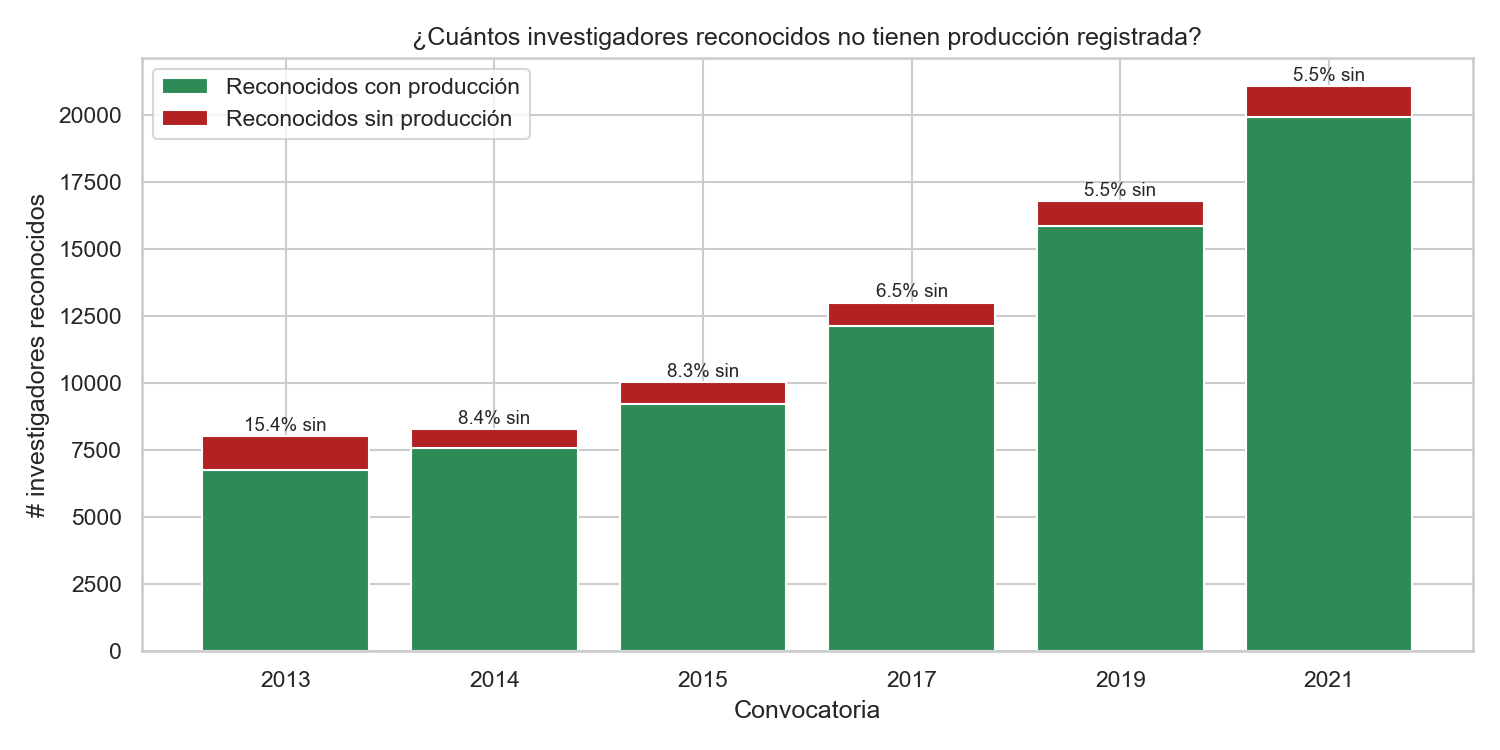
\includegraphics[width=0.92\linewidth]{../../artifacts/sprint5_produccion/fig06_reconocidos_sin_produccion.png}
\caption{Porcentaje de investigadores reconocidos que no aparecen como autores de ningún producto en su ventana de observación.}
\end{figure}

La interpretación más razonable de la caída es que la captura del campo de productos mejoró con el tiempo. En 2013 el sistema dejaba pasar reconocimientos sin enlace explícito a productos; en 2021, ese enlace es más sistemático. El 5{,}5\,\% remanente sigue siendo una pregunta abierta y vale la pena documentar caso a caso.

% =====================================================================
\section{Recomendaciones de política pública}\label{sec:recomendaciones}
% =====================================================================

Los hallazgos se agrupan en cuatro líneas operativas para MinCiencias.

\subsection{Calidad y gobernanza del dato}

\begin{enumerate}[label=A.\arabic*., leftmargin=*]
\item \textbf{Validación previa a la publicación.} Reglas mínimas: edad menor o igual a 100 años, fecha de convocatoria distinta de fecha de publicación, departamentos válidos contra lista DANE, género en valores cerrados. Costo: bajo. Beneficio: rankings públicos sin errores groseros.
\item \textbf{Adopción de la tabla maestra de instituciones.} Entregamos un primer borrador (211 IES canónicas, 91\,\% de cobertura). La recomendación es que MinCiencias lo adopte como estándar de captura: cuando un investigador reporte afiliación, el sistema sugiera o restrinja a entidades del catálogo canónico.
\item \textbf{Departamento de la institución como campo obligatorio.} El análisis geográfico institucional sólo fue posible por la tabla maestra que construimos manualmente. Si el formulario capturara el departamento de la institución, la información estaría disponible para todos por defecto.
\end{enumerate}

\subsection{Equidad y diversidad}

\begin{enumerate}[label=B.\arabic*., leftmargin=*]
\item \textbf{Captura obligatoria de variables de diversidad desde el formulario inicial.} Etnia, discapacidad y condición de víctima del conflicto deben ser campos obligatorios en todas las convocatorias, no sólo desde 2021. La captura puede ser de auto-reporte y respetar el derecho a no responder, pero la variable debe existir desde el origen.
\item \textbf{Comparación contra población educada como métrica oficial.} Los reportes sobre representación de minorías deberían usar como referente la composición de la población con educación superior, no la población total.
\item \textbf{Programas focalizados en regiones con baja retención local.} La evidencia del \ref{ssec:h7-geografia} muestra que Cundinamarca y Risaralda pierden cerca de un tercio de sus investigadores hacia otros departamentos. Los programas regionales pueden focalizarse allí.
\end{enumerate}

\subsection{Apertura y trazabilidad}

\begin{enumerate}[label=C.\arabic*., leftmargin=*]
\item \textbf{Captura sistemática de doble afiliación.} En todas las convocatorias, no sólo en 2019. La estructura del campo \texttt{inst\_filia} ya soporta listas separadas por pipe, pero el formulario sólo solicita una institución en la mayoría de las convocatorias.
\item \textbf{Apertura del padrón completo de ScienTI.} El cruce con el dataset de producción mostró que cerca de cincuenta mil autores firman productos sin estar en el padrón de reconocidos. Una parte sí tiene perfil en ScienTI pero no se postula. Abrir el padrón completo permitiría caracterizar mejor el sistema.
\item \textbf{Apertura del dataset de proyectos evaluados.} Cerrar el ciclo idea → proyecto → producto → reconocimiento.
\end{enumerate}

\subsection{Métricas alineadas con la realidad}

\begin{enumerate}[label=D.\arabic*., leftmargin=*]
\item \textbf{Productividad ajustada por categoría, área OCDE y género.} Los rankings agregados no son comparables sin ajustar por las dimensiones donde sabemos que hay sesgos sistemáticos. MinCiencias debería publicar tanto la métrica cruda como la métrica ajustada.
\item \textbf{Reporte de flujos investigador--institución.} Documentar dónde reside el investigador y dónde está su institución es información que el observatorio entrega; debería ser visible en los reportes oficiales.
\item \textbf{Calendario predecible de convocatorias.} La diferencia entre convocatorias varía entre uno y tres años. Esa variabilidad afecta análisis longitudinales y la planificación de los grupos de investigación.
\end{enumerate}

% =====================================================================
\section{Limitaciones y trabajo futuro}\label{sec:limitaciones}
% =====================================================================

\paragraph{Lo que la fuente no permite resolver.}
La identidad de los \num{48811} autores no reconocidos. Resolverlo requiere acceso al padrón completo de ScienTI o a registros académicos institucionales que no están en datos.gov.co.

\paragraph{Lo que la fuente permite pero no abordamos en profundidad.}
\begin{itemize}
\item Análisis intersectorial. Los hallazgos sobre género, territorio y diversidad se presentan por separado. La intersección merece un capítulo propio.
\item Extensión de la tabla maestra. La cobertura actual es del 91\,\%; la cola larga del 9\,\% se puede completar revisando la lista de \texttt{evidencias/ies\_pendientes\_revision.csv}.
\end{itemize}

\paragraph{Lo que requiere fuentes adicionales.}
\begin{itemize}
\item Comparación contra población con educación superior (DANE Encuesta de Calidad de Vida o GEIH).
\item Comparación con sistemas similares de la región (CONACYT México, ANID Chile, CONICET Argentina).
\item Vinculación con el sistema de financiación de proyectos para construir el ciclo idea--reconocimiento--producto.
\end{itemize}

\paragraph{Lo que está pendiente del propio proyecto.}
\begin{itemize}
\item Convocatoria 2023, no disponible al cierre.
\item Despliegue público del tablero en Streamlit Community Cloud.
\end{itemize}

% =====================================================================
\section{Conclusiones}\label{sec:conclusiones}
% =====================================================================

El sistema de reconocimiento de investigadores en Colombia, leído con los propios datos abiertos del Ministerio, muestra patrones que sólo aparecen cuando se combinan las dos fuentes oficiales y se examina la serie de seis convocatorias.

La calidad de los datos es mejorable con esfuerzo bajo: validaciones de rango, una tabla maestra de instituciones y captura obligatoria del departamento institucional resolverían los problemas más visibles. La tabla maestra que entregamos junto al informe (211 IES, 91\,\% de cobertura) puede servir de punto de partida.

La concentración territorial es estructural. Bogotá y Antioquia capturan la mitad del padrón. La novedad de este análisis es que la concentración no es uniforme cuando se mide en productos por capita: regiones medianas como Bolívar y Risaralda producen por encima de su tamaño. Y al cruzar residencia con institución aparece que Bogotá no sólo concentra, sino que absorbe: cerca de mil investigadores residen en otros departamentos pero trabajan en Bogotá.

La brecha de género es estructural por área OCDE y se replica en productividad. La cifra agregada de 40\,\% de mujeres oculta que en Ingeniería sigue siendo del 24\,\%, y que las mujeres reciben menos atribución de productos en cinco de seis grandes áreas. Diez años de convocatorias no muestran cierre.

La diversidad étnica, etaria y de víctimas del conflicto es invisible en cinco de seis convocatorias. Sólo en 2021 empieza a registrarse, y los grupos numéricamente importantes aparecen significativamente sub-representados.

El cruce entre reconocimiento y producción agrega información que las fuentes no daban por separado. La productividad escala con la categoría. Los Eméritos producen poco en su última ventana visible porque después de ser reconocidos quedan vitalicios y no se postulan más. Y un tercio de los autores que sostienen la producción contabilizada por MinCiencias no está en el padrón.

El código, los datasets de evidencia, la tabla maestra de instituciones y el tablero interactivo están publicados en el repositorio referenciado al inicio. Cualquiera puede reproducir las cifras o extender el análisis con fuentes adicionales.

% =====================================================================
\appendix
\section*{Anexos}
\addcontentsline{toc}{section}{Anexos}
\renewcommand{\thesubsection}{\Alph{subsection}}

\subsection{Catálogo de variables clave}

\subsubsection*{Dataset de investigadores (\texttt{bqtm-4y2h})}

\begin{tabularx}{\linewidth}{l X}
\toprule
\textbf{Variable} & \textbf{Descripción} \\
\midrule
\texttt{id\_persona\_pr} & Identificador único en ScienTI. \\
\texttt{id\_convocatoria} & Identificador numérico de la convocatoria (16--21). \\
\texttt{ano\_convo} & Fecha de la convocatoria (puede ser fecha de publicación). \\
\texttt{nme\_clasificacion\_pr} & Junior, Asociado, Senior, Emérito. \\
\texttt{nme\_gran\_area\_pr} & Gran área OCDE (nivel 1). \\
\texttt{nme\_genero\_pr} & Género del investigador. \\
\texttt{nme\_departamento\_res\_pr} & Departamento de residencia. \\
\texttt{inst\_filia} & Institución(es) de afiliación, separadas por \texttt{|}. \\
\texttt{id\_victima\_conflicto} & Indicador (Si/No), capturado desde 2021. \\
\texttt{txt\_grupo\_etnico} & Grupo étnico, capturado desde 2021. \\
\texttt{txt\_poblacion\_disca} & Condición de discapacidad, capturada desde 2021. \\
\texttt{edad\_anos\_pr} & Edad en años (22 outliers tratados en \ref{ssec:val-calidad}). \\
\bottomrule
\end{tabularx}

\subsubsection*{Dataset de producción (\texttt{33dq-ab5a})}

\begin{tabularx}{\linewidth}{l X}
\toprule
\textbf{Variable} & \textbf{Descripción} \\
\midrule
\texttt{id\_persona\_pd} & Identificador del autor. Cruza con \texttt{id\_persona\_pr}. \\
\texttt{id\_convocatoria} & Ventana de observación. \\
\texttt{id\_producto\_pd} & Identificador único del producto. \\
\texttt{nme\_categoria\_pd} & Categoría detallada (ej. ``Artículos de investigación Con Calidad A1''). \\
\texttt{nme\_tipo\_medicion\_pd} & Tipo de medición MinCiencias (Apropiación, Formación, Nuevo conocimiento). \\
\texttt{fcreacion\_pd} & Fecha real de creación del producto. \\
\texttt{cod\_grupo\_gr} & Código del grupo de investigación. \\
\texttt{nme\_grupo\_gr} & Nombre del grupo. \\
\bottomrule
\end{tabularx}

\subsection{Modelo dimensional en DuckDB}

El modelo estrella consolidado tiene como tablas centrales:

\begin{itemize}
\item \texttt{fact\_clasificacion}: una fila por (investigador, convocatoria).
\item \texttt{fact\_produccion}: una fila por (autor, convocatoria, producto).
\item \texttt{vw\_investigador\_x\_produccion}: vista que cruza ambas tablas por \texttt{id\_persona} y \texttt{id\_convocatoria}.
\item Dimensiones: \texttt{dim\_convocatoria}, \texttt{dim\_categoria}, \texttt{dim\_area}, \texttt{dim\_territorio}, \texttt{dim\_formacion}, \texttt{dim\_institucion}, \texttt{dim\_producto}, \texttt{dim\_grupo}.
\end{itemize}

\subsection{Reproducibilidad}

\begin{lstlisting}[language=bash,caption={Reproducción completa.}]
git clone https://github.com/Victor-Diaz-Usta/Min_ciencias.git
cd Min_ciencias
poetry install

# Descargas (la segunda demora ~10 min, ~1.2 GB)
python -m src.ingesta.minciencias
python -m src.ingesta.produccion

# Hallazgos del observatorio
python scripts/sprint6_validacion_calidad.py    # Atipicos de edad
python scripts/sprint2_panel_longitudinal.py    # Trayectoria longitudinal
python scripts/sprint2_matrices_transicion.py
python scripts/sprint6_sankey_categoria.py      # Sankeys de categoria
python scripts/sprint2_territorial.py
python scripts/sprint6_tabla_maestra_ies.py     # Tabla maestra IES
python scripts/sprint6_geografia_institucional.py
python scripts/sprint6_sankey_territorial.py
python scripts/sprint2_genero_ocde.py
python scripts/sprint3_redes.py
python scripts/sprint3_grafo_interactivo.py
python scripts/sprint4_diversidad.py
python scripts/sprint5_produccion.py
python scripts/sprint6_ocde_composicion.py

# Modelo dimensional
python scripts/sprint2_duckdb.py
python scripts/sprint5_duckdb.py

# Tablero interactivo
streamlit run streamlit_app.py

# Manual reproducible
jupyter notebook docs/manual.ipynb
\end{lstlisting}

\subsection{Fuentes consultadas}

\begin{itemize}
\item \textbf{datos.gov.co --- Investigadores reconocidos por convocatoria}. \\ \url{https://www.datos.gov.co/resource/bqtm-4y2h.csv}
\item \textbf{datos.gov.co --- Producción de Grupos de Investigación}. \\ \url{https://www.datos.gov.co/resource/33dq-ab5a.csv}
\item \textbf{MinCiencias --- Datos abiertos}. \\ \url{https://minciencias.gov.co/ciudadano/datosabiertos}
\item \textbf{ScienTI Colombia --- Plataforma de perfiles de investigadores}. \\ \url{https://www.minciencias.gov.co/scienti}
\item \textbf{DANE --- Censo Nacional de Población y Vivienda 2018}. \\ \url{https://www.dane.gov.co/index.php/estadisticas-por-tema/demografia-y-poblacion/censo-nacional-de-poblacion-y-vivenda-2018}
\item \textbf{Unidad para las Víctimas --- Registro Único de Víctimas (RUV)}. \\ \url{https://www.unidadvictimas.gov.co/es/registro-unico-de-victimas-ruv/37394}
\item \textbf{Repositorio del observatorio}. \url{\repoUrl}
\end{itemize}

\vspace{2em}
\begin{center}
\rule{0.5\textwidth}{0.5pt}\\[0.4em]
{\footnotesize\color{rule}Cierre del informe \,$\cdot$\, \universidad \,$\cdot$\, \periodo}
\end{center}

\end{document}
